\documentclass[11pt]{article}
% -----------------------------------------------------------------------------
% Revision notes for MS CPENG-8674 (major review, October 2026):
% enhanced case study, datasets, corrections of the SciML model and validation.
% Code: MODULES/review29oct_fixed  |  Figures: ./figures
% -----------------------------------------------------------------------------
\usepackage[a4paper,margin=2.5cm]{geometry}
\usepackage{amsmath,amssymb,bm}
\usepackage{graphicx}
\usepackage{booktabs,multirow,array}
\usepackage{xcolor}
\usepackage{caption,subcaption}
\usepackage{float}
\usepackage{enumitem}
\usepackage{lineno}
\usepackage{titlesec}
\usepackage{tikz}
\usetikzlibrary{decorations.pathmorphing,arrows.meta,calc,positioning}
\usepackage[colorlinks=true,linkcolor=red!70!black,citecolor=red!70!black,urlcolor=magenta]{hyperref}

\linespread{1.45}
\linenumbers
\captionsetup{labelfont=rm,font=small,labelsep=colon}
\captionsetup[figure]{name=FIG.}
\captionsetup[table]{name=TABLE}
\titleformat{\section}{\normalfont\sffamily\bfseries\MakeUppercase}{}{0pt}{}
\titleformat{\subsection}{\normalfont\bfseries}{}{0pt}{}
\setcounter{secnumdepth}{0}

\newcommand{\m}{\mathbf{m}}
\newcommand{\z}{\mathbf{z}}
\newcommand{\f}{\mathbf{f}}
\newcommand{\Kh}{\hat{\mathbf{K}}_{\mathrm{G}}}
\newcommand{\MG}{\mathbf{M}_{\mathrm{G}}}
\newcommand{\Lelbo}{\mathcal{L}_{\mathrm{ELBO}}}
\newcommand{\qz}{q_{\bm{\zeta}_{\bm\theta}}(\z|\m)}

\title{\sffamily\bfseries Uncertainty-aware damage identification in short-span bridges via physics-informed variational autoencoder\\[4pt]
\large Revision notes: case study, datasets, corrections of the SciML model and validation}
\author{Ana Fernandez-Navamuel; \'Angel J.\ Omella; Diego Zamora-Sanchez; David Pardo}
\date{Revision of MS CPENG-8674 --- \today}

\begin{document}
\maketitle

\section{Introduction}

The reviewers raised three main concerns about the numerical study of the submitted manuscript: the structural model
was too simple (a five-element, simply supported beam), the test data came from the same model used for training,
and measurement noise was the only source of uncertainty. In addition, a detailed inspection of the code revealed
implementation errors that affected the estimated posteriors and the reference (ground-truth) posteriors used to
assess them. This document describes how we addressed these issues. We keep the methodology of the submitted version
(encoder, Gaussian copula sampling layer, differentiable eigenvalue decoder, and the loss of Eq.~(10)) and follow its
notation.

The document has four parts. The first describes the enhanced case study: a bridge on elastic bearings, a finer
finite element (FE) model to generate the test data, and the sources of uncertainty that the decoder does not
represent. The second describes the datasets and explains how these uncertainty sources enter the inference. The
third describes the corrections of the implementation. The fourth describes how we compute the reference posteriors
and compare them with the VAE estimates. Table~\ref{tab:reviewers} relates each change to the reviewers' comments;
the code is available in \texttt{MODULES/review29oct\_fixed}.

\begin{table}[H]
\centering\small
\caption{Correspondence between the changes and the reviewers' comments.}
\label{tab:reviewers}
\begin{tabular}{p{2.4cm}p{12cm}}
\toprule
Comment & Change \\
\midrule
R1.1, R1.7 & The test observations come from a 50-element FE model with the same damage zones and sensors as the
10-element model embedded in the decoder. \\
R1.2, R3.1 & Temperature, mass and within-zone stiffness variability are present in all simulated data; their effect
is included in the likelihood as a calibrated model discrepancy. \\
R1.3 & Coverage is evaluated at several nominal levels using the exact marginal distributions of the VAE. \\
R1.6 & The training set is balanced across healthy, mildly damaged and localized damage scenarios; we report the
false-alarm rate. \\
R2.2, R2.3 & The bridge rests on elastic bearings, each with its own stiffness reduction factor. \\
R3.2 & Hyperparameters and the final model are selected on the validation set only. \\
R3.3 & The prior of the ELBO (uniform) is independent of the sampling density used to generate the training set. \\
R3.4 & We quantify how the observed quantities and the number of modes control the width of the posterior. \\
R3.7 & The ELBO is estimated with $H=6$ samples per observation. \\
\bottomrule
\end{tabular}
\end{table}

% =============================================================================
\section{Enhanced case study}
% =============================================================================

\subsection{Bridge on elastic bearings}

Following Reviewer~2, we replace the simply supported beam of Eq.~(2) by a beam resting on elastic bearings
(Fig.~\ref{fig:fe}). Each bearing is represented by a vertical spring of stiffness $k_v$ and a rotational spring of
stiffness $k_r$. Damage can now occur in the deck and in the bearings. We divide the deck into five zones of equal
length and assign one stiffness reduction factor to each zone and one to each bearing. The damage condition vector
therefore has seven components,
\begin{equation}
\z = \{z_1,\dots,z_5,\,z_{b,L},\,z_{b,R}\}^\top\in\mathcal{S}=[z_{\mathrm{lb}},1]^{7},\qquad z_{\mathrm{lb}}=0.45 ,
\end{equation}
which define the seven-dimensional latent space of the VAE. The dimension of the latent space depends only on the
number of zones and bearings, not on the number of finite elements: each zone $k$ may contain several elements
$e\in\mathcal{Z}_k$, all of them scaled by the same factor $z_k$. The updated global stiffness matrix of Eq.~(5) thus
becomes
\begin{equation}
\Kh(\z) = \sum_{k=1}^{5} z_k \sum_{e\in\mathcal{Z}_k}\mathbf{K}_{e,\mathrm{G}}
        + z_{b,L}\,\mathbf{K}_{b,L} + z_{b,R}\,\mathbf{K}_{b,R},
\label{eq:Kz}
\end{equation}
where $\mathbf{K}_{b,L}$ and $\mathbf{K}_{b,R}$ contain the nominal bearing stiffnesses $k_{v0}$ and $k_{r0}$ at the
vertical and rotational DOFs of the end nodes. Since the bearings are elastic, no DOF is removed and
$n_{\mathrm{dof}}=2(n_{\mathrm{el}}+1)$. The mode shapes are observed at the six zone boundaries by vertical
accelerometers, regardless of the mesh. Table~\ref{tab:specs} summarizes the main specifications.

\begin{figure}[H]
\centering
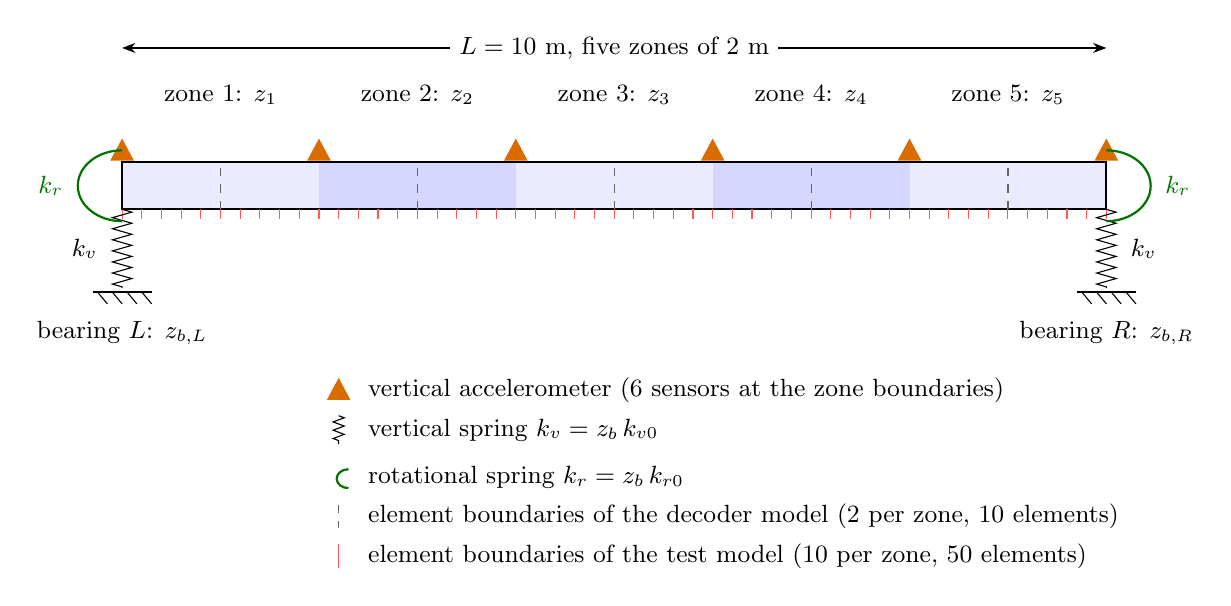
\begin{tikzpicture}[x=1.25cm,y=1cm,>=Stealth,font=\small]
  % deck zones
  \foreach \i/\c in {0/blue!8,1/blue!16,2/blue!8,3/blue!16,4/blue!8}{
    \fill[\c] (2*\i,0) rectangle (2*\i+2,0.6);
    \node at (2*\i+1,1.45) {zone $\the\numexpr\i+1\relax$: $z_{\the\numexpr\i+1\relax}$};
  }
  \draw[thick] (0,0) rectangle (10,0.6);
  % meshes
  \foreach \x in {1,3,5,7,9} \draw[dashed,gray!80!black] (\x,0) -- (\x,0.6);
  \foreach \k in {0,...,50} \draw[red!65] (\k*0.2,-0.12) -- (\k*0.2,0);
  % accelerometers (triangles)
  \foreach \x in {0,2,4,6,8,10}
    \fill[orange!85!black] (\x-0.12,0.62) -- (\x+0.12,0.62) -- (\x,0.9) -- cycle;
  % bearings
  \foreach \x/\lab/\a/\b in {0/{L}/90/270,10/{R}/-90/90}{
    \draw[decorate,decoration={zigzag,segment length=4,amplitude=3.5}] (\x,0) -- (\x,-1.0);
    \draw[thick] (\x-0.3,-1.05) -- (\x+0.3,-1.05);
    \foreach \h in {-0.25,-0.1,0.05,0.2} \draw (\x+\h,-1.05) -- (\x+\h+0.1,-1.2);
    \draw[thick,green!45!black] (\x,0.3) ++(\a:0.45) arc (\a:\b:0.45);
    \node[align=center,anchor=north] at (\x,-1.3) {bearing $\lab$: $z_{b,\lab}$};
  }
  \node[anchor=east] at (-0.15,-0.5) {$k_v$};
  \node[anchor=east,green!45!black] at (-0.5,0.3) {$k_r$};
  \node[anchor=west] at (10.15,-0.5) {$k_v$};
  \node[anchor=west,green!45!black] at (10.5,0.3) {$k_r$};
  % dimensions
  \draw[<->] (0,2.05) -- (10,2.05) node[midway,fill=white] {$L=10$ m, five zones of 2 m};
  % legend
  \begin{scope}[shift={(2.2,-2.3)}]
    \fill[orange!85!black] (-0.12,-0.12) -- (0.12,-0.12) -- (0,0.16) -- cycle; \node[anchor=west] at (0.2,0) {vertical accelerometer (6 sensors at the zone boundaries)};
    \draw[decorate,decoration={zigzag,segment length=3,amplitude=2}] (0,-0.32) -- (0,-0.68); \node[anchor=west] at (0.2,-0.5) {vertical spring $k_v=z_b\,k_{v0}$};
    \draw[thick,green!45!black] (0.1,-1.0) arc (90:270:0.12); \node[anchor=west] at (0.2,-1.1) {rotational spring $k_r=z_b\,k_{r0}$};
    \draw[dashed,gray!80!black] (0,-1.45) -- (0,-1.75); \node[anchor=west] at (0.2,-1.6) {element boundaries of the decoder model (2 per zone, 10 elements)};
    \draw[red!65] (0,-1.95) -- (0,-2.25); \node[anchor=west] at (0.2,-2.1) {element boundaries of the test model (10 per zone, 50 elements)};
  \end{scope}
\end{tikzpicture}
\caption{Bridge on elastic bearings. The seven unknowns are the stiffness reduction factors of the five deck zones
($z_1,\dots,z_5$) and of the two bearings ($z_{b,L}$, $z_{b,R}$, which scale both springs of each bearing). The VAE
decoder uses a 10-element model; the test observations are generated with a 50-element model.}
\label{fig:fe}
\end{figure}

\begin{table}[H]
\centering\small
\caption{Main specifications of the case study.}
\label{tab:specs}
\begin{tabular}{p{4.6cm}p{10.2cm}}
\toprule
Deck & $L=10$ m, $E=210$ GPa, $\rho=7850$ kg/m$^3$, $A=0.005$ m$^2$, $I=8.33\times10^{-6}$ m$^4$ \\
Bearings (each end) & $k_{v0}=1.5\times10^{8}$ N/m, $k_{r0}=5\times10^{6}$ N\,m/rad \\
Unknowns (latent space) & $\z\in[0.45,1]^7$: five deck zones and two bearings \\
Decoder model & 10 elements (2 per zone), 22 DOFs, nominal mass and modulus \\
Test model & 50 elements (10 per zone), 102 DOFs \\
Observations & first $n_m=5$ frequencies and vertical mode shapes at $n_n=6$ sensors ($d=35$) \\
\bottomrule
\end{tabular}
\end{table}

\subsection{Discretization of the decoder and of the test model}

Reviewer~1 asked us to test the trained VAE on observations generated by a finer mesh, keeping the same damage zones
and sensors. Such a test is only meaningful if the model embedded in the decoder is accurate enough. With one element
per zone, as in the submitted version, the fifth frequency differs by 13\% from a converged model
(Table~\ref{tab:mesh}). This error is much larger than the measurement noise, so the VAE would fail on finer-mesh data
for reasons unrelated to the method. With two elements per zone, the error drops below 0.5\%. We therefore embed a
10-element model in the decoder and generate the test observations with a 50-element model. The remaining
discrepancy between both models is small and is handled as described in the next section.

\begin{table}[H]
\centering\small
\caption{Relative error (\%) of the natural frequencies of the healthy bridge with respect to a 200-element model.}
\label{tab:mesh}
\begin{tabular}{lccccc}
\toprule
Model & $f_1$ & $f_2$ & $f_3$ & $f_4$ & $f_5$ \\
\midrule
5 elements (submitted version) & 0.04 & 0.32 & 1.15 & 2.42 & 13.33 \\
10 elements (decoder) & 0.003 & 0.02 & 0.08 & 0.22 & 0.48 \\
50 elements (test model) & 0.000 & 0.000 & 0.000 & 0.000 & 0.001 \\
\midrule
Frequencies of the 50-element model [Hz] & 6.68 & 18.58 & 36.65 & 60.84 & 91.09 \\
\bottomrule
\end{tabular}
\end{table}

\subsection{Sources of uncertainty not represented by the decoder}

In practice, the measured modal properties of a bridge do not depend only on its stiffness. Reviewers~1 and~3 asked us
to consider other sources of variability. We include three of them in every simulated structure:
\begin{itemize}[leftmargin=*]
\item \emph{Temperature}, which changes the elastic modulus of the whole deck by the same factor $1+\delta_T$, with
$\delta_T\sim\mathcal{N}(0,0.03^2)$.
\item \emph{Mass uncertainty} (non-structural mass, pavement), as a factor $1+\mu_e$ on the mass of each element, with
$\mu_e\sim\mathcal{N}(0,0.02^2)$.
\item \emph{Spatial variability of stiffness} within each zone, as a factor $1/(1+\varepsilon_e)$ on each element,
with $\varepsilon_e\sim\mathcal{N}(0,0.025^2)$ and zero mean inside the zone, so that the equivalent stiffness of the
zone remains exactly $z_k$.
\end{itemize}
The element matrices of a simulated (``true'') structure are therefore
\begin{equation}
\mathbf{K}_e^{\mathrm{true}} = \frac{(1+\delta_T)\,z_{k(e)}}{1+\varepsilon_e}\,\mathbf{K}_e,\qquad
\mathbf{M}_e^{\mathrm{true}} = (1+\mu_e)\,\mathbf{M}_e .
\label{eq:true}
\end{equation}
These effects are deliberately \emph{not} included in the decoder, which remains the eigenvalue solver of the nominal
10-element model, as in the submitted methodology. The next section explains how the inference accounts for them.

% =============================================================================
\section{Datasets and likelihood}
% =============================================================================

\subsection{How unmodelled variability enters the inference}

The decoder computes the modal properties $\mathbf{g}(\z)$ of the nominal model for a given damage condition. The
measured modal properties, however, also reflect temperature, mass, mesh refinement and measurement noise. We write
the observations as
\begin{equation}
\m = \mathbf{g}(\z) + \underbrace{\mathbf{b} + \bm\epsilon_{\mathrm{model}}}_{\text{temperature, mass, mesh}}
     + \bm\epsilon_{\mathrm{meas}} ,
\label{eq:discrepancy}
\end{equation}
where $\mathbf{b}$ is a systematic bias, $\bm\epsilon_{\mathrm{model}}$ a random model discrepancy and
$\bm\epsilon_{\mathrm{meas}}$ the measurement noise. The stiffness factors $\z$ are not meant to absorb the
discrepancy. If the loss ignored it, a frequency drop caused by a warm day could only be explained by reducing some
$z_k$, producing a false damage detection with an overconfident posterior. Instead, the discrepancy is part of the
likelihood: we estimate the statistics of $\mathbf{b}+\bm\epsilon_{\mathrm{model}}+\bm\epsilon_{\mathrm{meas}}$ by
simulation and use them to weight the data terms of the loss (Eq.~\ref{eq:elbo}). This approach is standard in
Bayesian FE model updating and leaves the architecture unchanged.

The calibration of the likelihood has two important consequences. First, the observations are treated as less
precise than the measurement noise alone would suggest, which widens the posterior consistently with what the decoder
cannot represent. Second, temperature changes all frequencies together, so the frequency errors are strongly
correlated across modes. The likelihood therefore recognizes a uniform shift of all frequencies as a plausible
temperature effect, whereas a shift with a localized pattern, together with changes in the mode shapes, points to
damage.

\subsection{Calibration of the likelihood}

We simulate 6\,000 structures over the design of experiments described below. For each of them, we compare the modal
properties of the 50-element structure of Eq.~\eqref{eq:true} with those of the decoder at the same $\z$. For the
logarithms of the frequencies, the mean difference gives the bias $\mathbf{b}$, which ranges from $-0.05\%$ (mode~1)
to $-0.53\%$ (mode~5) and is due to the mesh. Their covariance, plus the identification noise, gives the matrix
$\bm\Sigma_f$. The resulting standard deviation is 1.6\% for every mode, and the correlation between modes is about
0.6, due to temperature. For the vertical mode shapes, the deviation from the decoder shapes (measured through the
MAC) gives a standard deviation $s_{v,j}$ per mode between 2.8\% and 3.9\% of the unit-norm shape.

We verify the calibration on independent test data: at the true damage condition, the average value of each likelihood
term must equal its theoretical value. The ratios lie between 0.98 and 1.01 (Fig.~\ref{fig:calib}), which confirms
that the likelihood describes the actual deviations between the observations and the decoder.

\begin{figure}[H]
\centering
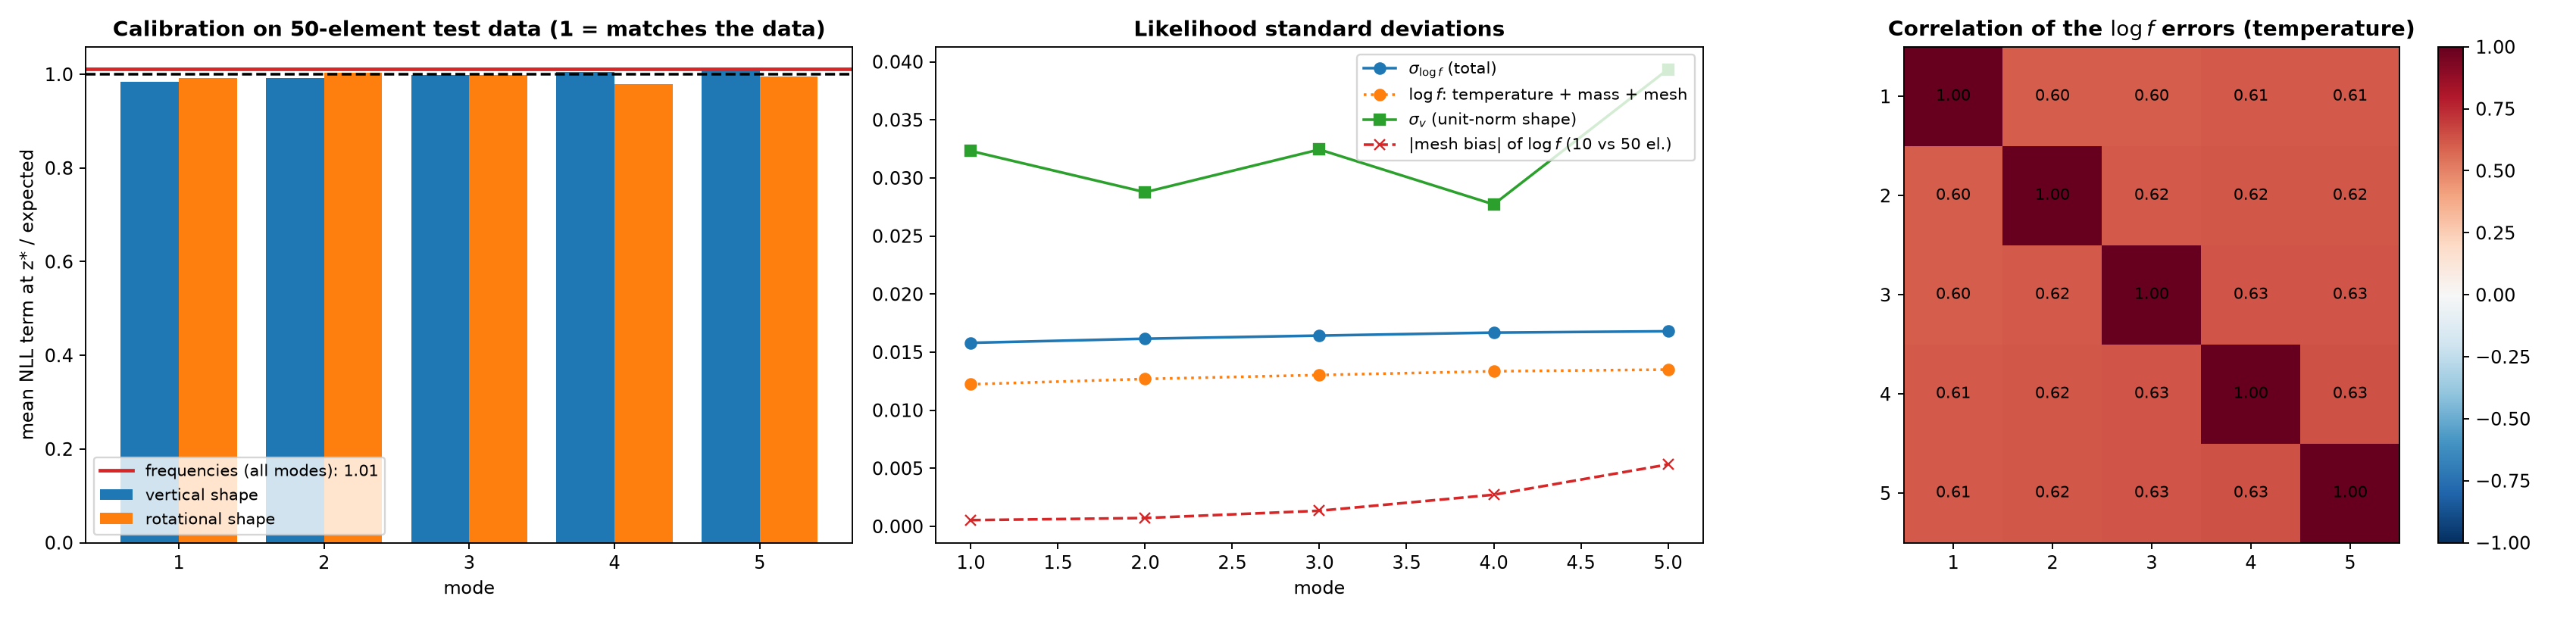
\includegraphics[width=\textwidth]{figures/Fig_likelihood_calibration.png}
\caption{Calibration of the likelihood against the 50-element test structure. Left: average likelihood terms at the
true state divided by their theoretical value (1 means calibrated). Centre: standard deviations of the
log-frequencies and of the vertical mode shapes. Right: correlation between the log-frequency errors of different
modes, caused by temperature.}
\label{fig:calib}
\end{figure}

\subsection{Design of experiments}

The submitted version sampled every stiffness reduction factor from $\mathcal{U}[0.5,1]$, so most samples had all
elements damaged simultaneously (Reviewer~1, comment~6). The new design of experiments (DoE) represents realistic and
balanced scenarios. Each sample belongs to one of the categories of Table~\ref{tab:doe}. Within each category, every
damage location (five zones and two bearings), or combination of locations, appears the same number of times. The
damaged factors are drawn from $[0.45,0.95)$ with Latin hypercube stratification, which covers severe, moderate and
mild damage uniformly, and the undamaged factors are drawn from $[0.95,1]$. As a result, every parameter is damaged in
33.2\% of the training samples (Fig.~\ref{fig:doe}).

\begin{table}[H]
\centering\small
\caption{Scenario categories of the design of experiments.}
\label{tab:doe}
\begin{tabular}{lcl}
\toprule
Category & Share & Damaged parameters \\
\midrule
Healthy & 10\% & none \\
Single damage & 30\% & one (each of the seven locations equally often) \\
Double damage & 25\% & two (all 21 pairs) \\
Triple damage & 15\% & three (all 35 triples) \\
Multiple damage & 10\% & four or five (all 56 combinations) \\
Uniform & 10\% & $\z\sim\mathcal{U}[0.45,1]^7$, to cover the whole support of the prior \\
\bottomrule
\end{tabular}
\end{table}

\begin{figure}[H]
\centering
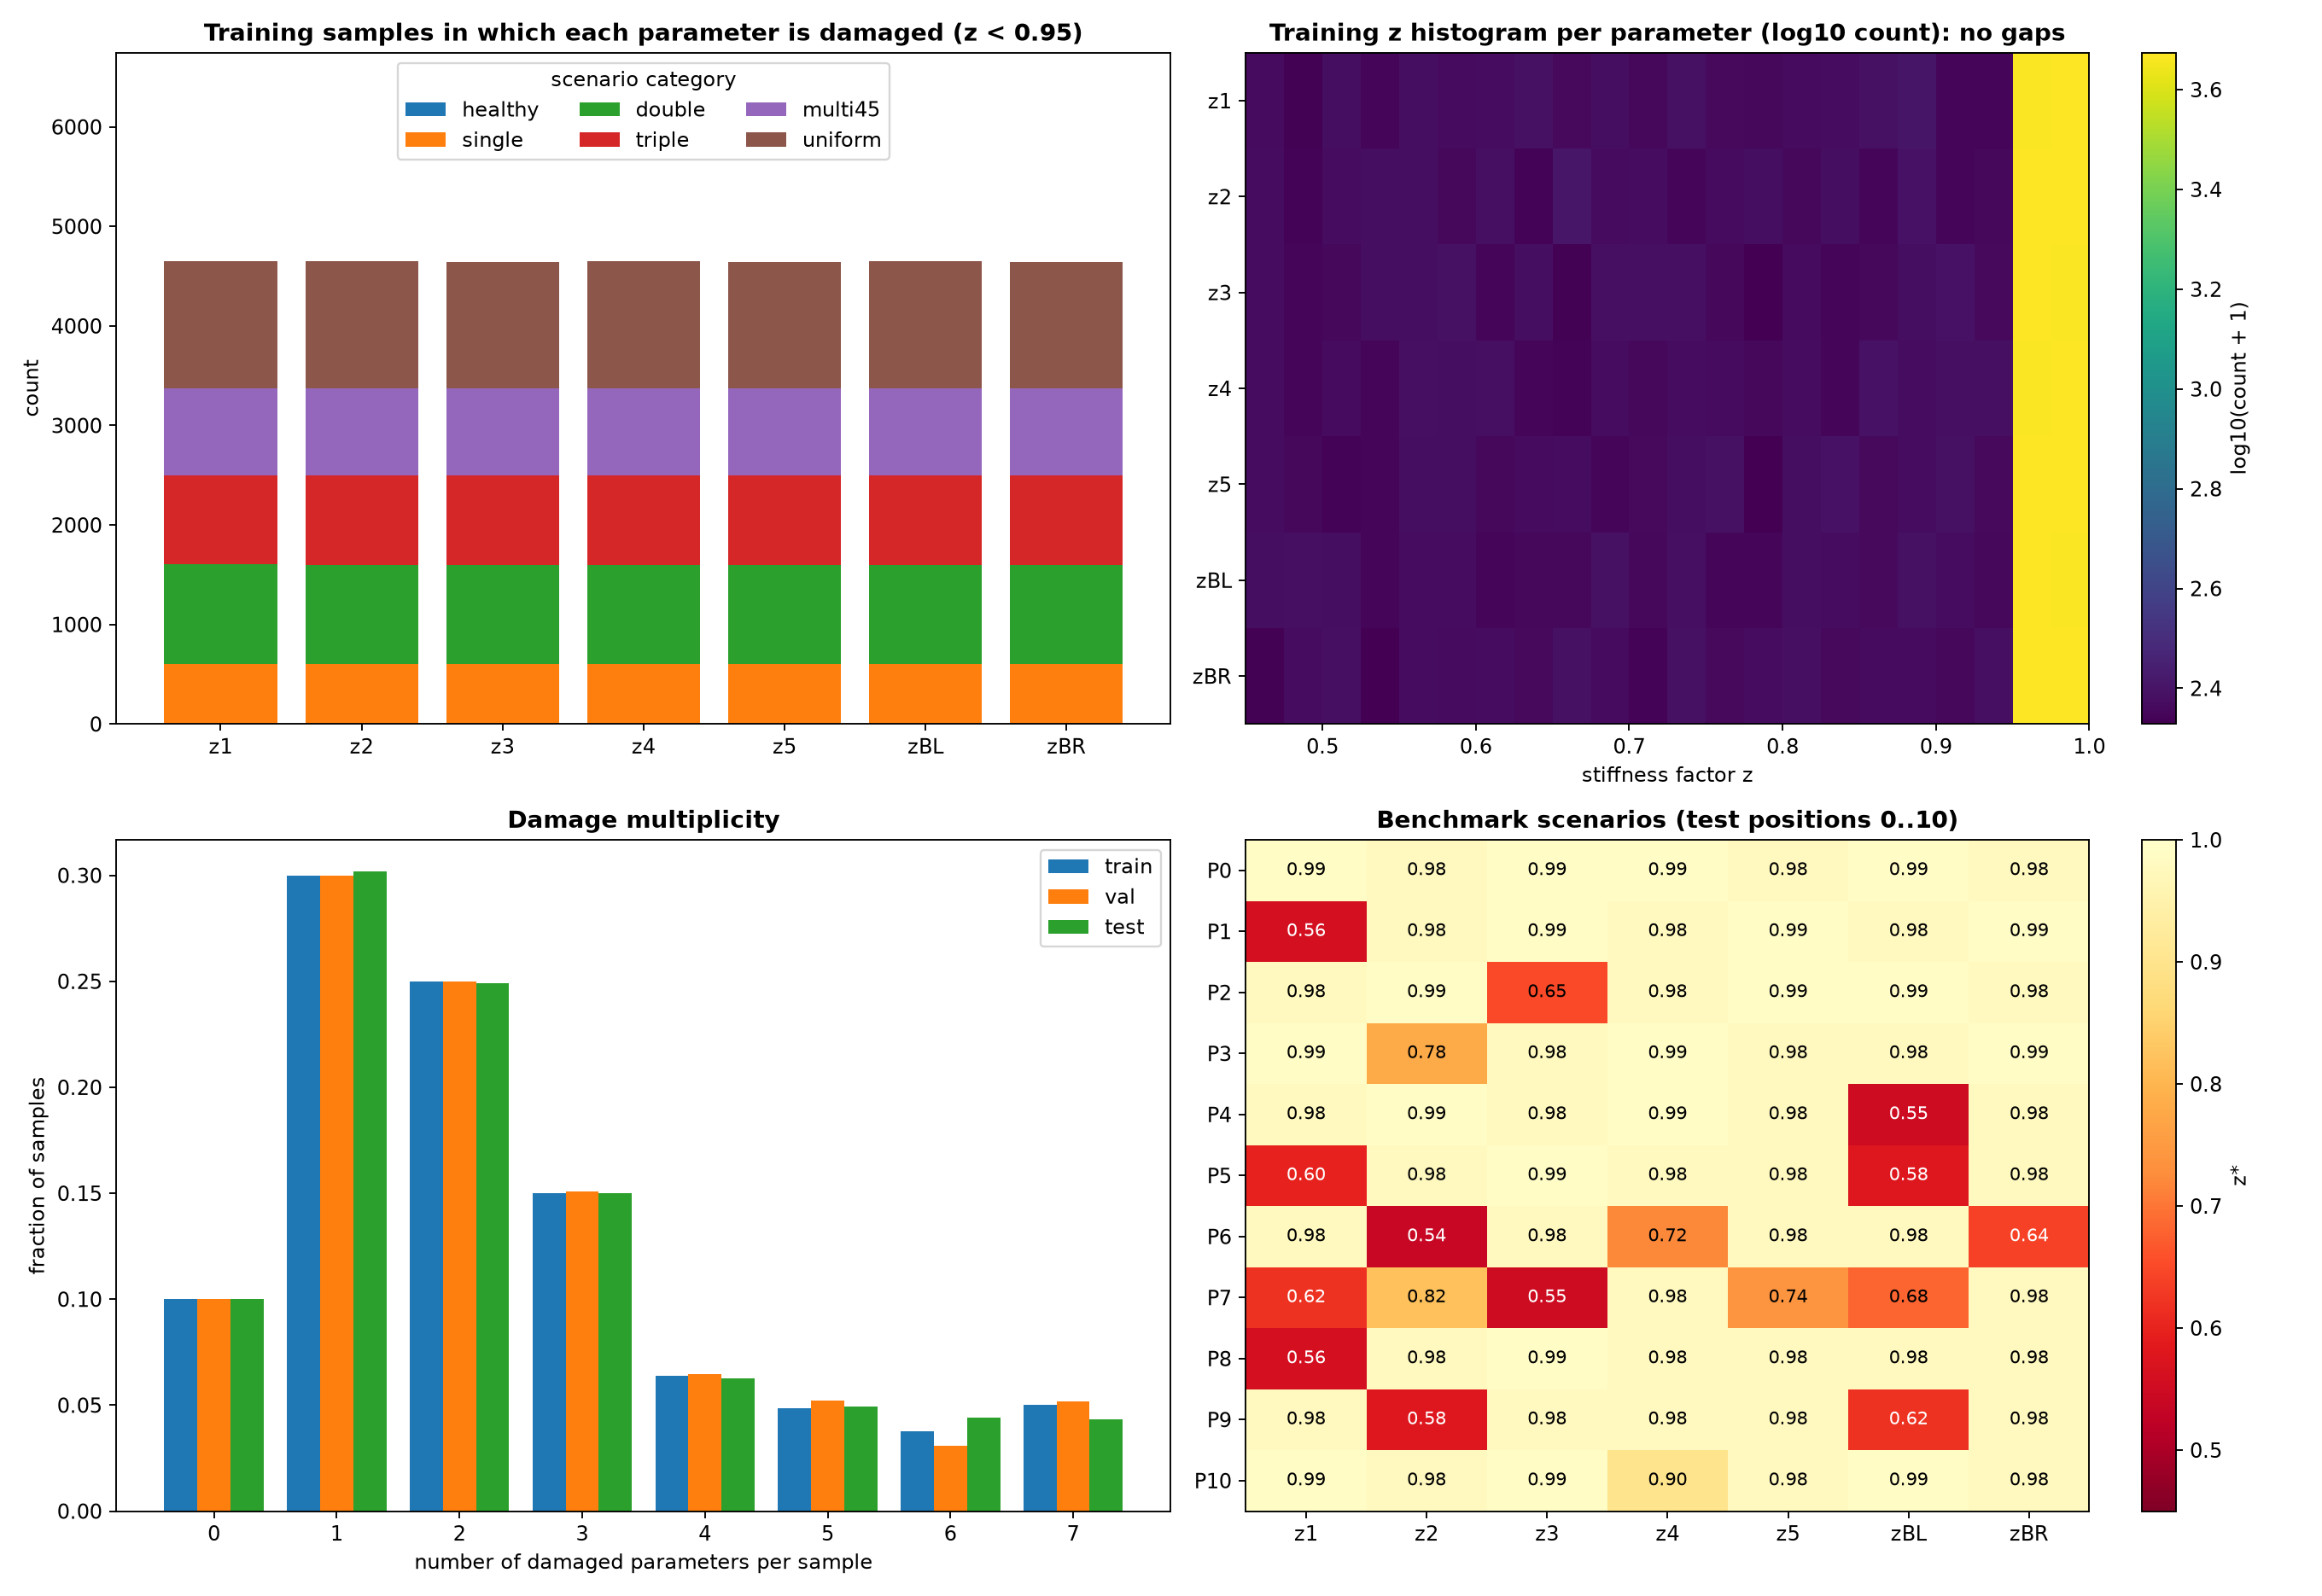
\includegraphics[width=0.95\textwidth]{figures/Fig_DoE_balance.png}
\caption{Design of experiments: number of training samples in which each parameter is damaged, by category;
histogram of the stiffness reduction factors; number of damaged parameters per sample; and the eleven benchmark test
scenarios.}
\label{fig:doe}
\end{figure}

\subsection{Training, validation and test datasets}

The three datasets differ in their purpose and in the model that generates them (Table~\ref{tab:datasets}). The
training and validation observations are generated with the 10-element model, and the test observations with the
50-element model, so that the VAE is evaluated on data from a more refined model than the one it was trained with. All
of them include temperature, mass and within-zone variability (Eq.~\ref{eq:true}). We solve the generalized
eigenvalue problem of each structure, keep the first five modes, and add measurement noise as in the submitted
version: a multiplicative noise of 1\% on the frequencies, and an additive noise on the mode shapes with a standard
deviation of 5\% of the peak amplitude of each mode. The noisy shapes are normalized to unit length and their sign is
aligned with the healthy shapes.

We observe the vertical mode shapes only, because accelerometers measure vertical motion; the observation vector is
$\m=\mathrm{flat}(\{\f,\bm\Phi\})\in\mathbb{R}^{35}$. The first eleven test samples are benchmark scenarios
(Fig.~\ref{fig:doe}, bottom right): ten of them keep the damage conditions of the submitted version and one adds a
case of mild damage ($z_4=0.90$). All of them are plain simulations of a single structure.

\begin{table}[H]
\centering\small
\caption{Datasets.}
\label{tab:datasets}
\begin{tabular}{p{5.6cm}>{\centering}p{2.7cm}>{\centering}p{2.7cm}>{\centering\arraybackslash}p{2.9cm}}
\toprule
 & Training & Validation & Test \\
\midrule
Number of samples & 14\,000 & 2\,400 & 1\,200 (11 benchmarks) \\
Model that generates the data & 10 elements & 10 elements & 50 elements \\
Temperature, mass, within-zone variability & yes & yes & yes \\
Measurement noise (1\% frequencies, 5\% shapes) & yes & yes & yes \\
Purpose & minimize the ELBO & select the model & evaluate the model \\
\bottomrule
\end{tabular}
\end{table}

\subsection{Information content and width of the posterior}

The width of the posterior reflects how much information the observations contain. Table~\ref{tab:information}
shows the standard deviation of the exact posterior for three benchmark scenarios under different measurement setups.
When the rotations are also measured at every node with low noise, as in the intermediate version of our code, the
posterior is very concentrated and a deterministic estimate would be almost as informative. Observing the vertical
mode shapes only, with realistic noise and model discrepancy, yields posteriors with substantial uncertainty, which
varies across scenarios and parameters. Using fewer modes widens them further (Reviewer~3, comment~4).

\begin{table}[H]
\centering\small
\caption{Standard deviation of the exact posterior marginals (range over the seven parameters) for benchmarks P3,
P5 and P9.}
\label{tab:information}
\begin{tabular}{lc}
\toprule
Observed quantities and noise (frequencies / shapes) & Posterior standard deviation \\
\midrule
Frequencies, vertical and rotational shapes, 1.5\% / 3\% & 0.013--0.028 \\
Frequencies and vertical shapes, 1.5\% / 3\% & 0.016--0.044 \\
Frequencies and vertical shapes, 2.5\% / 5\% & 0.024--0.073 \\
Frequencies and vertical shapes, 2.5\% / 5\%, three modes & 0.031--0.153 \\
\midrule
Adopted setup (Table~\ref{tab:specs}), all eleven benchmarks & 0.02--0.13 \\
\bottomrule
\end{tabular}
\end{table}

Figure~\ref{fig:gt} shows the exact posteriors of four benchmark scenarios with the adopted setup. The marginals are
asymmetric, the bearings are the most uncertain parameters (95\% credible intervals up to 0.47 wide), and several
pairs of parameters are clearly correlated. For example, in P9 a stiffer deck near the left support can compensate a
weaker left bearing ($z_1$ and $z_{b,L}$), and in P7 the same happens at the right end ($z_5$ and $z_{b,R}$). The true
damage condition lies within the 95\% credible interval for six or seven of the seven parameters in every scenario.

\begin{figure}[H]
\centering
\begin{subfigure}{0.49\textwidth}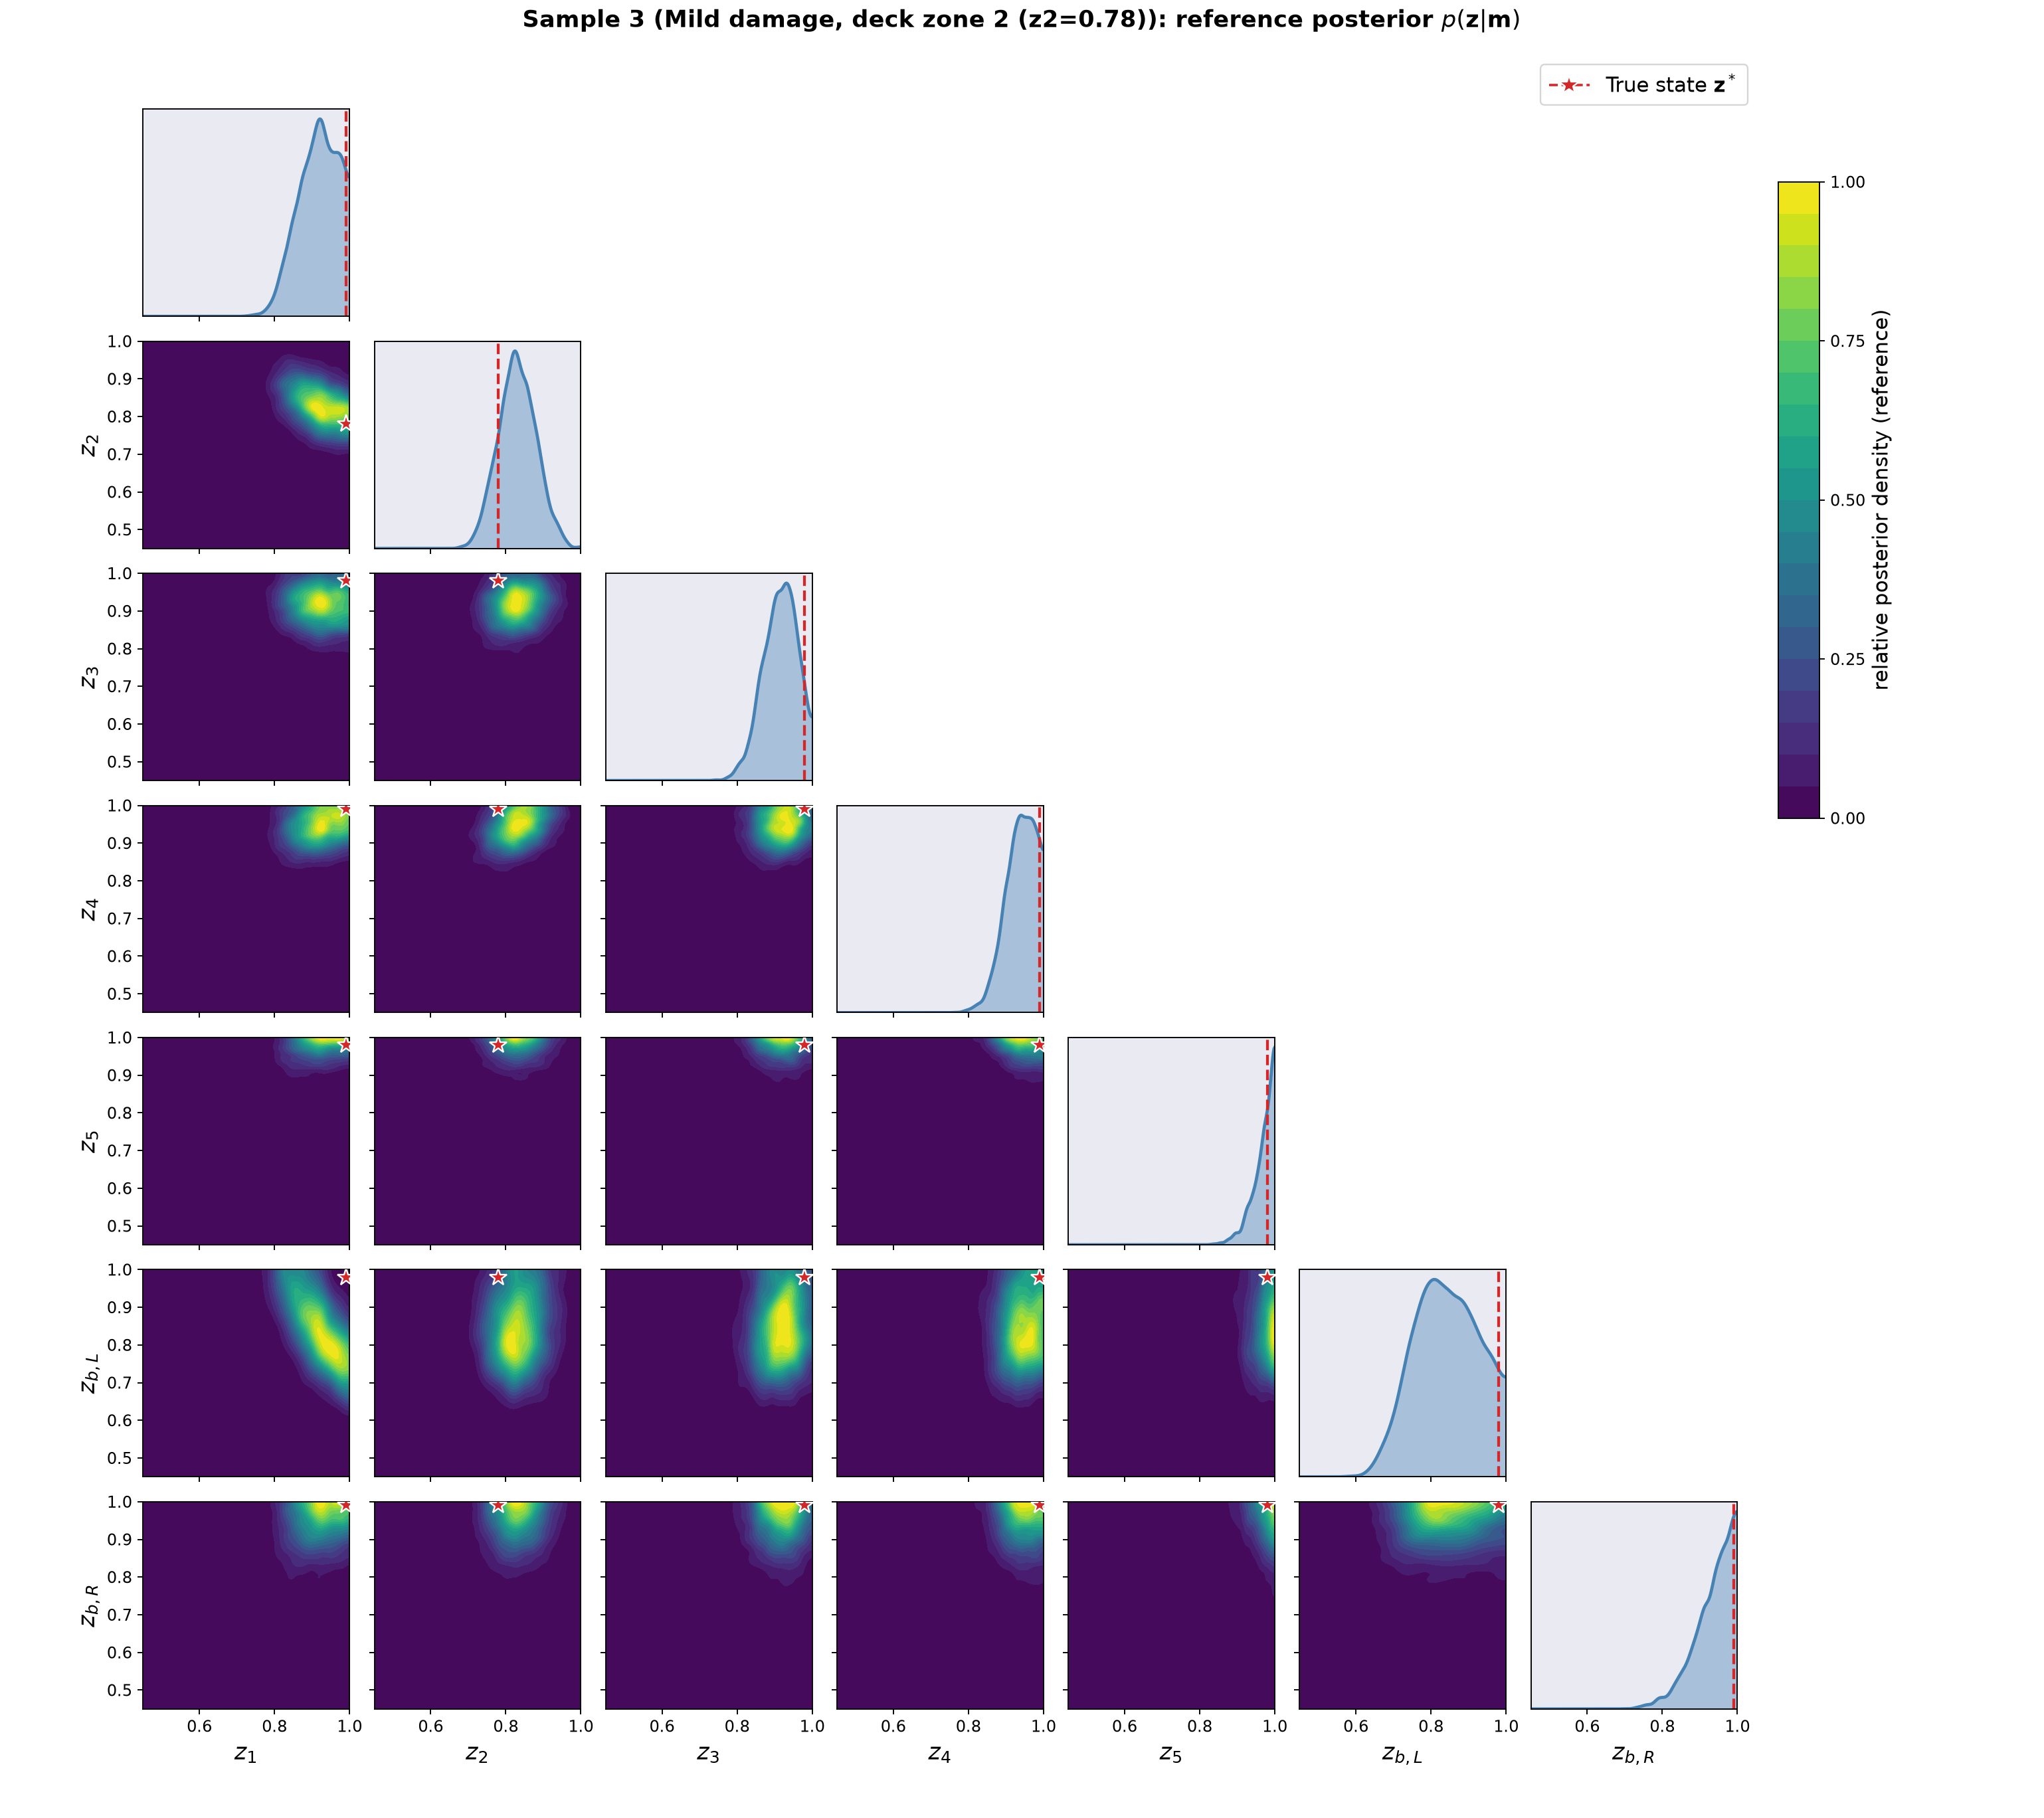
\includegraphics[width=\textwidth]{figures/GT_realistic_P3.png}\caption{P3: mild damage in zone 2 ($z_2=0.78$)}\end{subfigure}
\begin{subfigure}{0.49\textwidth}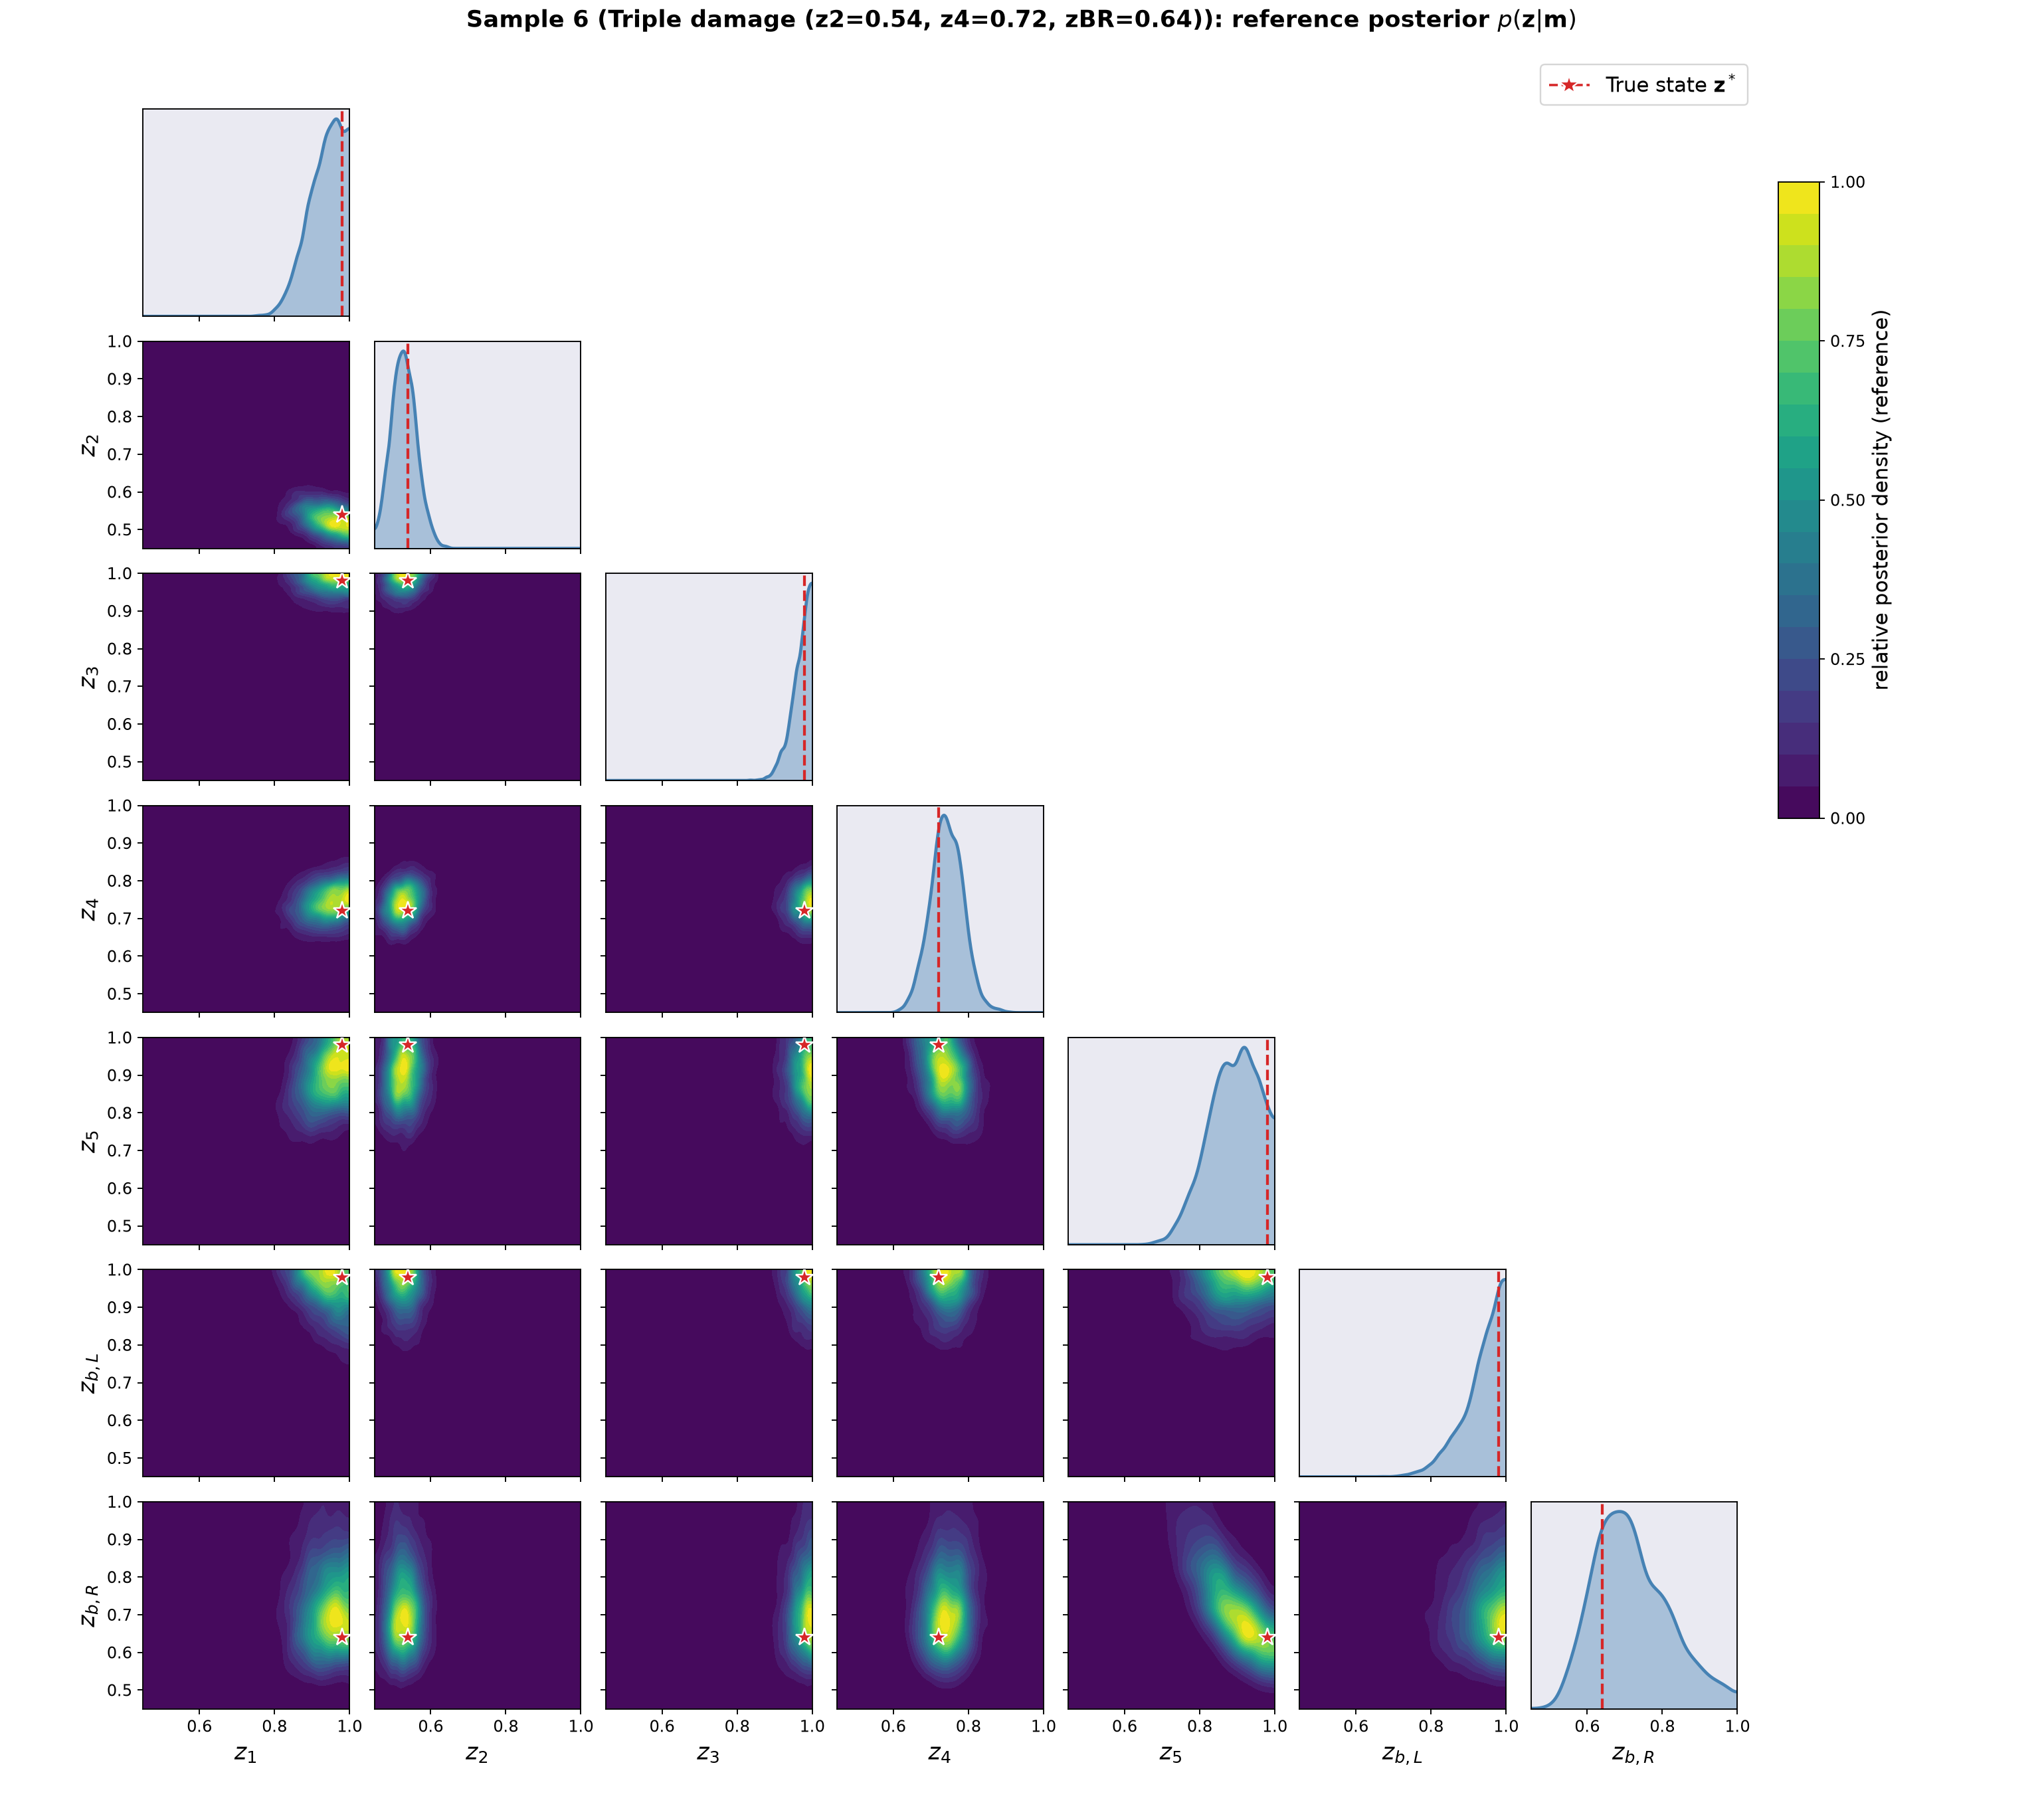
\includegraphics[width=\textwidth]{figures/GT_realistic_P6.png}\caption{P6: $z_2=0.54$, $z_4=0.72$, $z_{b,R}=0.64$}\end{subfigure}\\[4pt]
\begin{subfigure}{0.49\textwidth}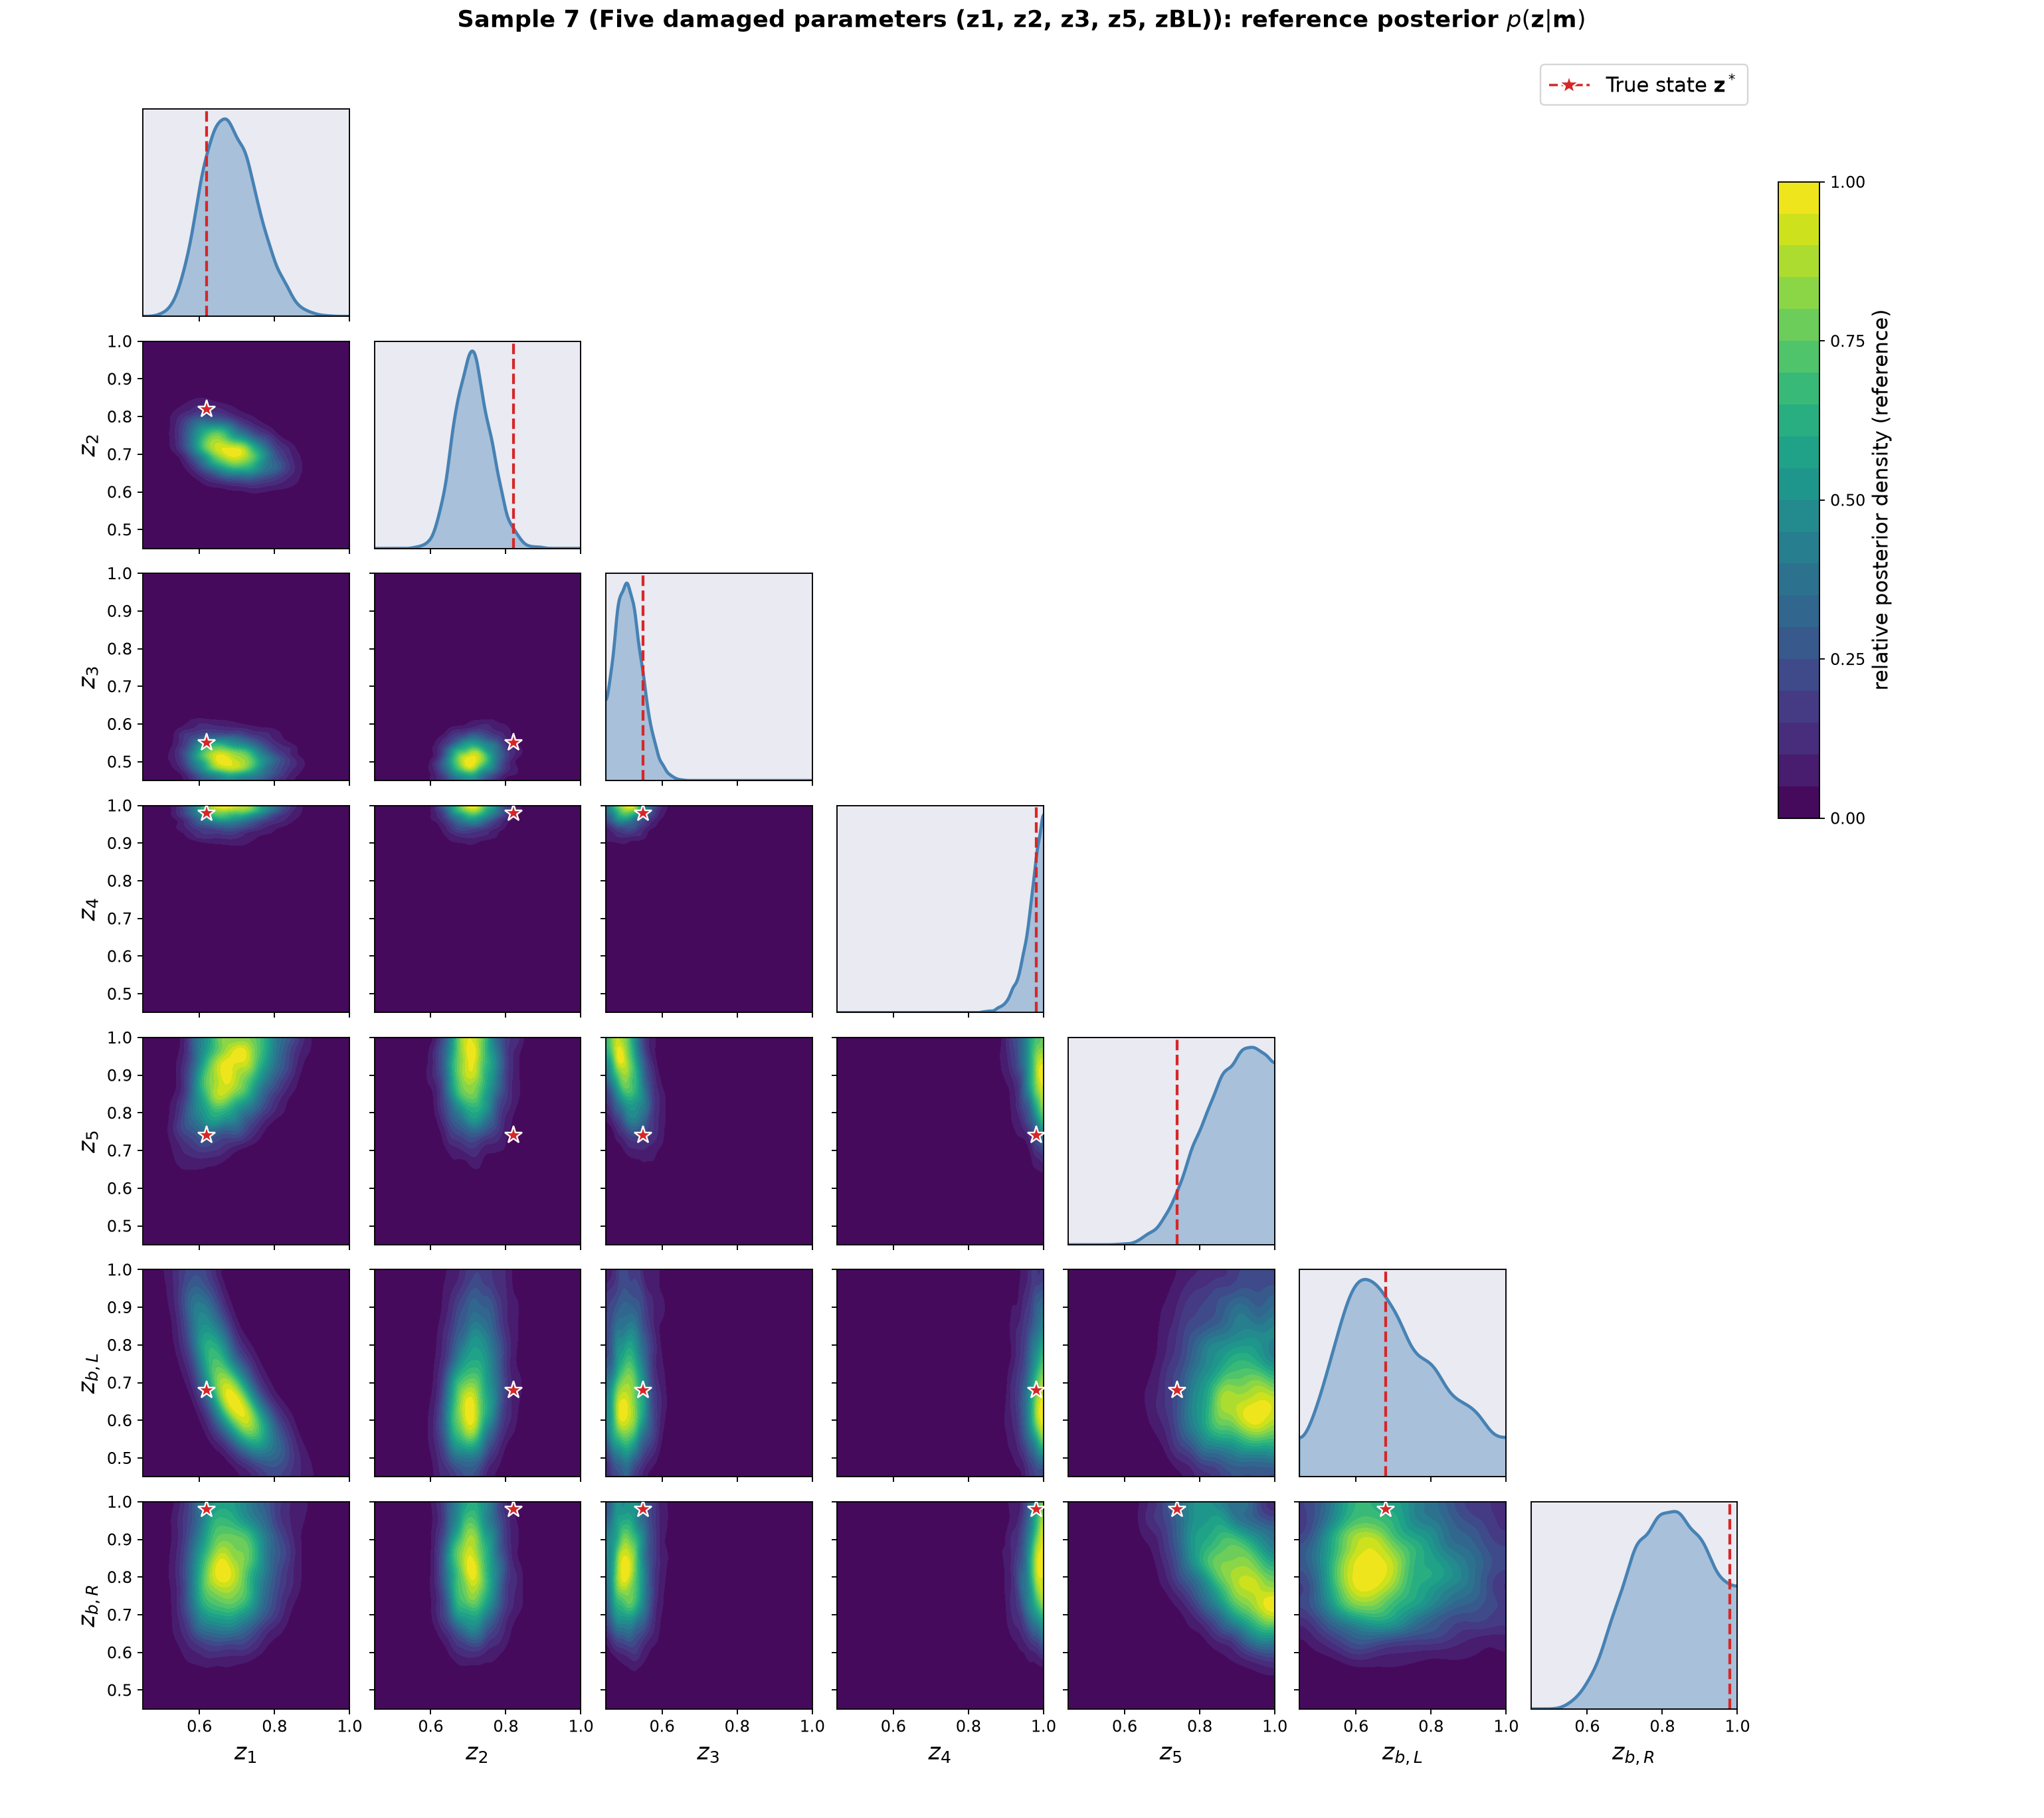
\includegraphics[width=\textwidth]{figures/GT_realistic_P7.png}\caption{P7: five damaged parameters}\end{subfigure}
\begin{subfigure}{0.49\textwidth}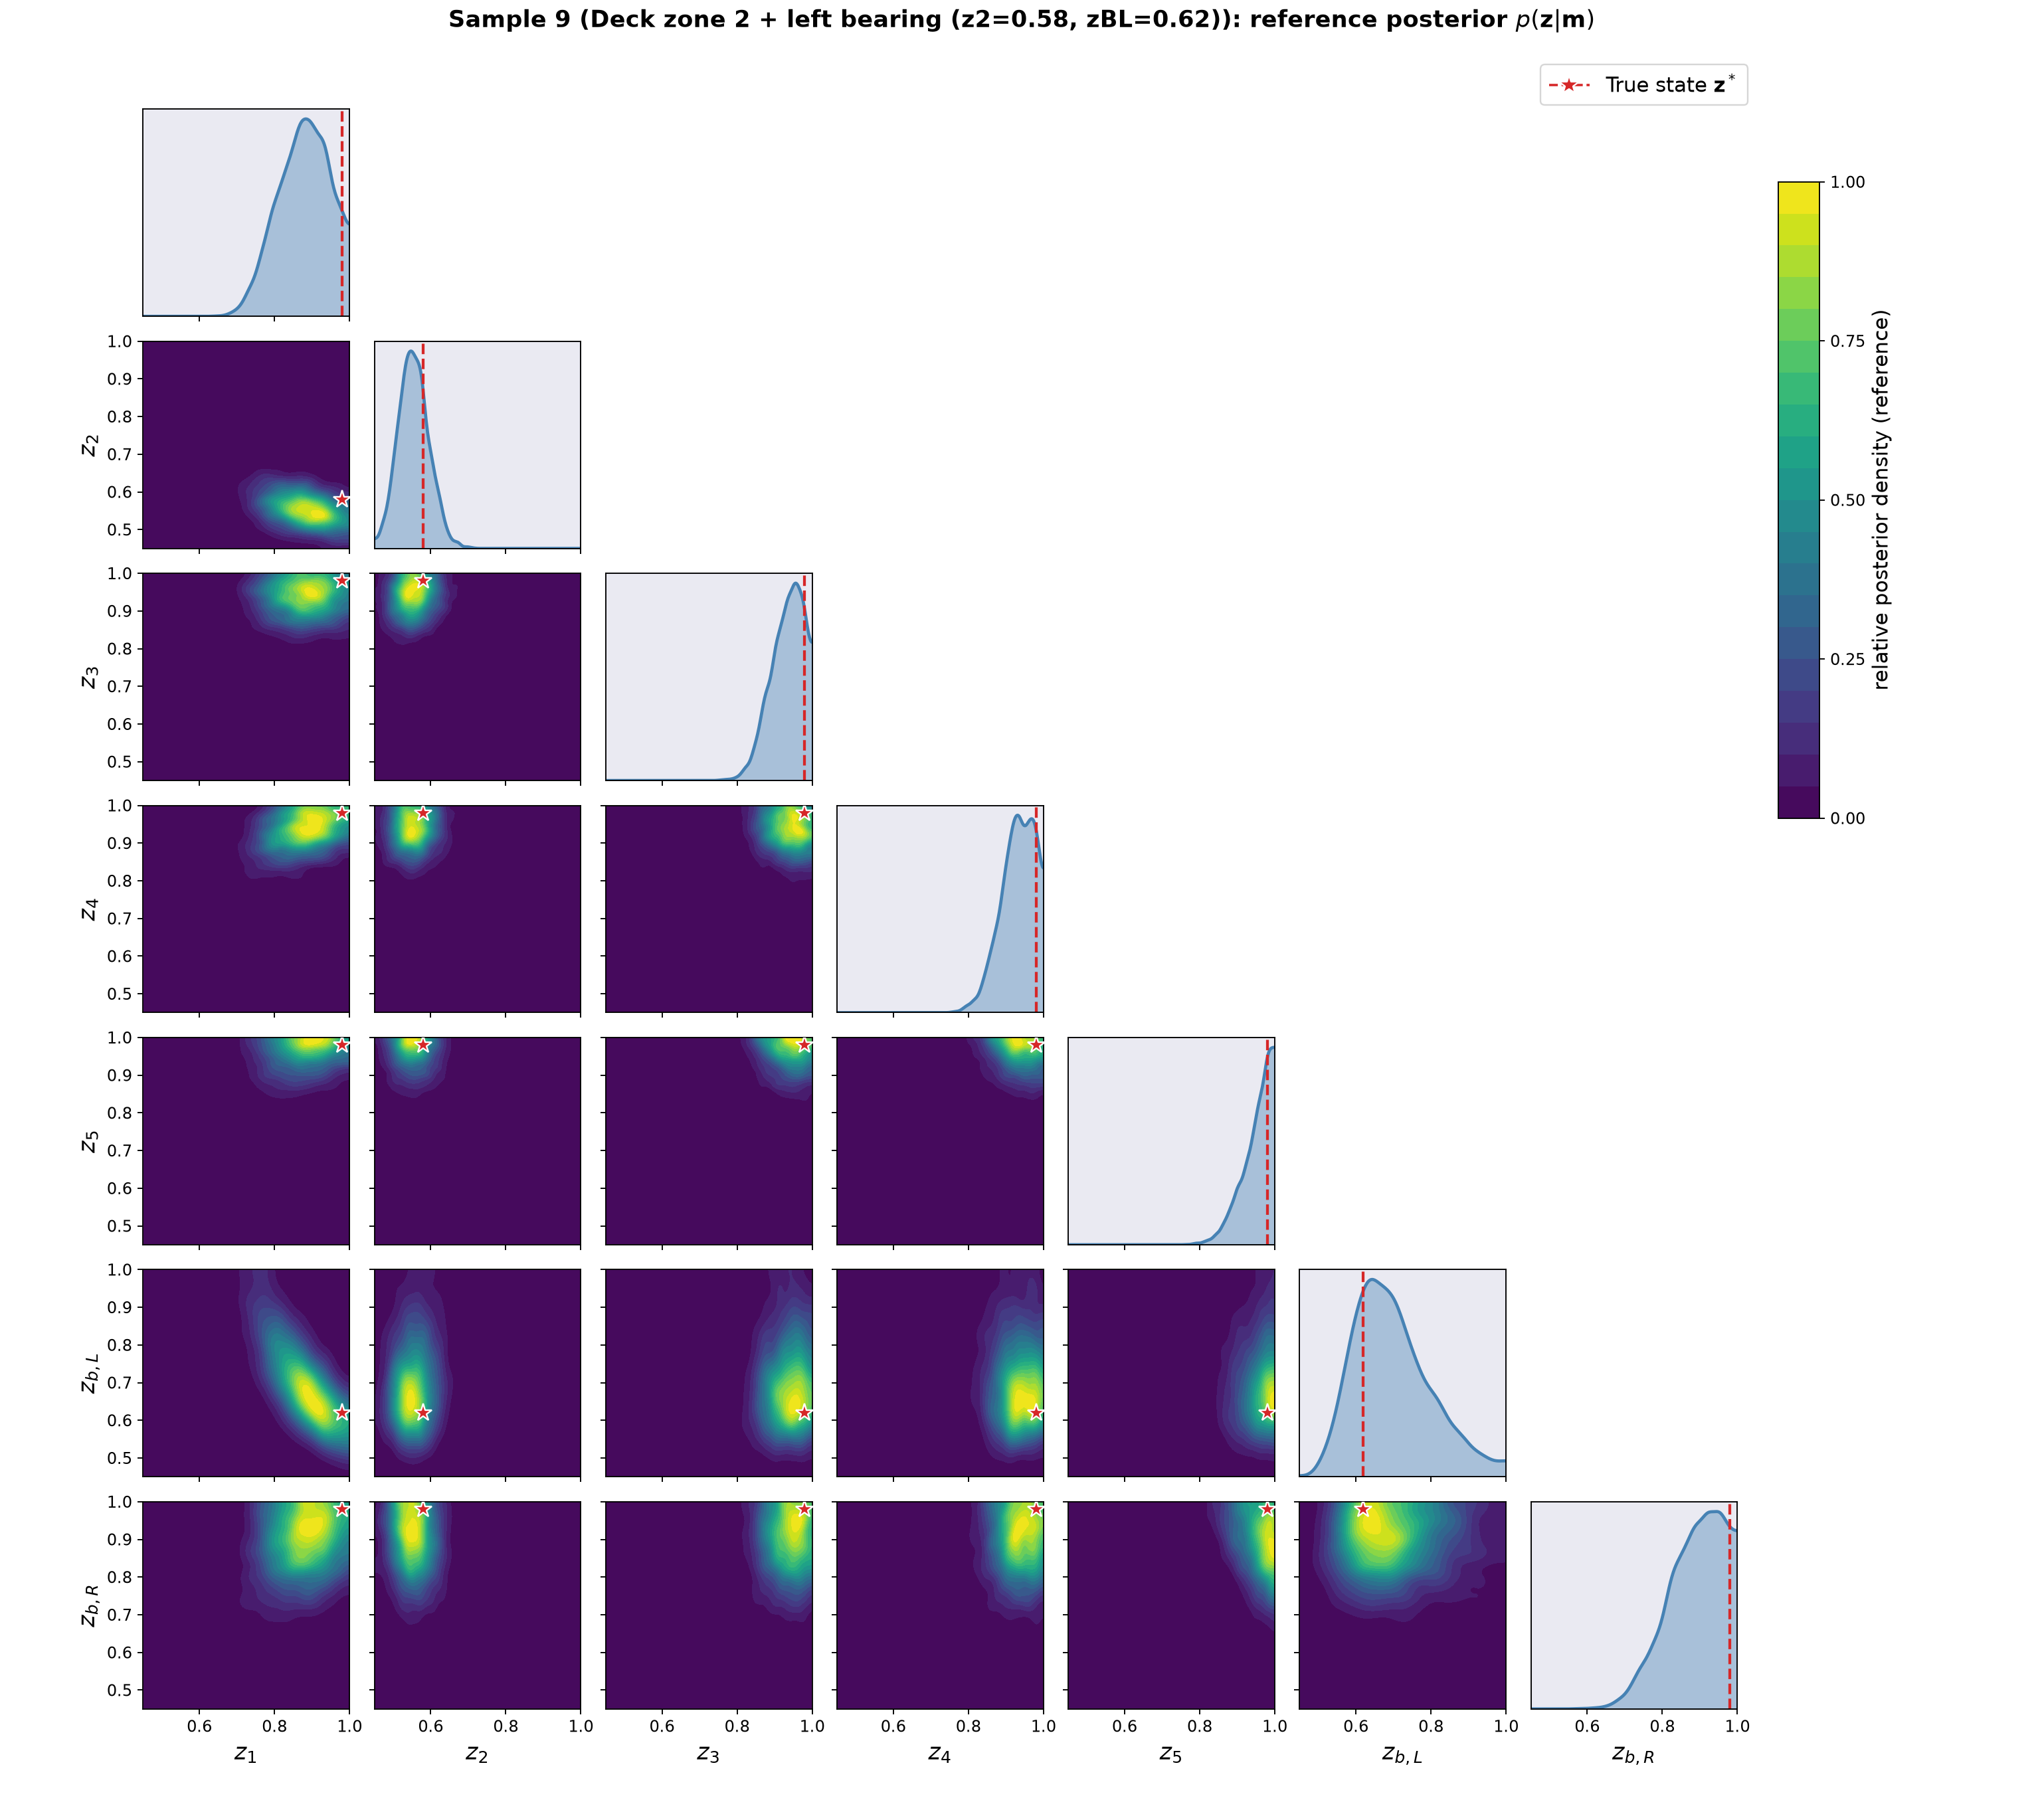
\includegraphics[width=\textwidth]{figures/GT_realistic_P9.png}\caption{P9: zone 2 and left bearing}\end{subfigure}
\caption{Exact posteriors $p(\z|\m_t)$ of four benchmark scenarios, computed from 50-element test observations. The
red star marks the true damage condition.}
\label{fig:gt}
\end{figure}

% =============================================================================
\section{Corrections of the SciML model}
% =============================================================================

The methodology of the submitted version is preserved. Following the limitation identified in its conclusions, the
truncated Gaussian marginals are replaced by mixtures of $K=3$ Kumaraswamy distributions, which are bounded and can
represent multimodal marginals. During the revision we found several errors in the implementation that made the
estimated posteriors unreliable. This section describes them, the corrected formulation of the loss, and the
verification of the corrected code.

\subsection{Errors found in the previous implementation}

The most important error concerned the sign of the PDF term. The ELBO requires the expected log-density of the
approximate posterior, $\mathcal{L}_{\mathrm{PDF}}=\mathbb{E}_q[\log\qz]$, which penalizes posteriors that are too
concentrated. The code implemented the opposite sign, so minimizing the loss rewarded posteriors that were as
concentrated as possible. The only limit was a clipping of $\log q$ at $+50$: the logged PDF term stayed exactly at
this limit for most of the training (Fig.~\ref{fig:old}a), and the encoder reached it by making the copula correlation
matrices nearly singular. This explains the thin, ridge-like joint densities observed in the previous results.

Three further issues affected the results. An auxiliary penalty pushed the samples away from $z=1$, where the
posterior of every undamaged parameter is located; consequently, undamaged parameters were underestimated by 0.02 to
0.06, while damaged ones were overestimated by 0.06 to 0.15. The gradients of the Kumaraswamy sampling layer were
clipped in several places, and the learning rate decreased by four orders of magnitude during training, which
effectively stopped the optimization after a few hundred epochs. Finally, the previous reference posterior was not a
valid posterior: part of its evaluation points were drawn around the true damage condition, the corresponding
correction weights were only partially applied, and its likelihood used a manually tuned temperature. As a result, it
was four to five times wider than the exact posterior (Fig.~\ref{fig:old}b), which made the VAE estimates look too
narrow by comparison.

\begin{figure}[H]
\centering
\begin{subfigure}{\textwidth}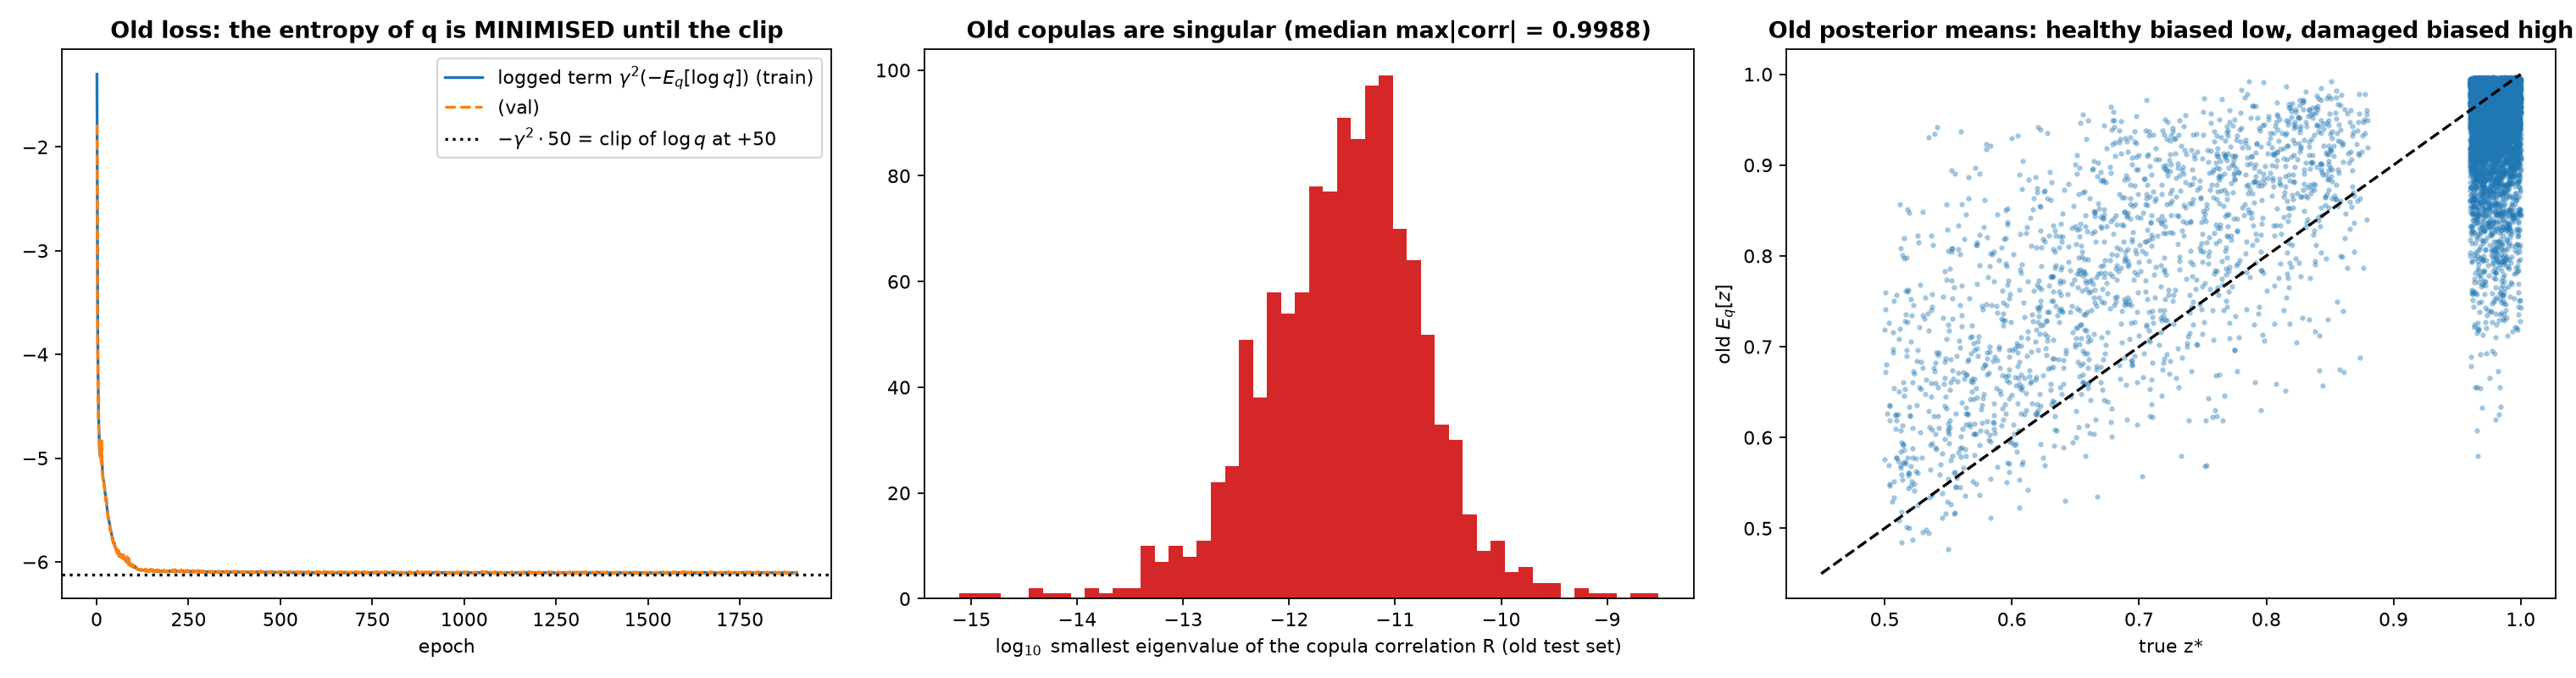
\includegraphics[width=\textwidth]{figures/Fig_old_training_and_copula.png}\caption{}\end{subfigure}\\
\begin{subfigure}{\textwidth}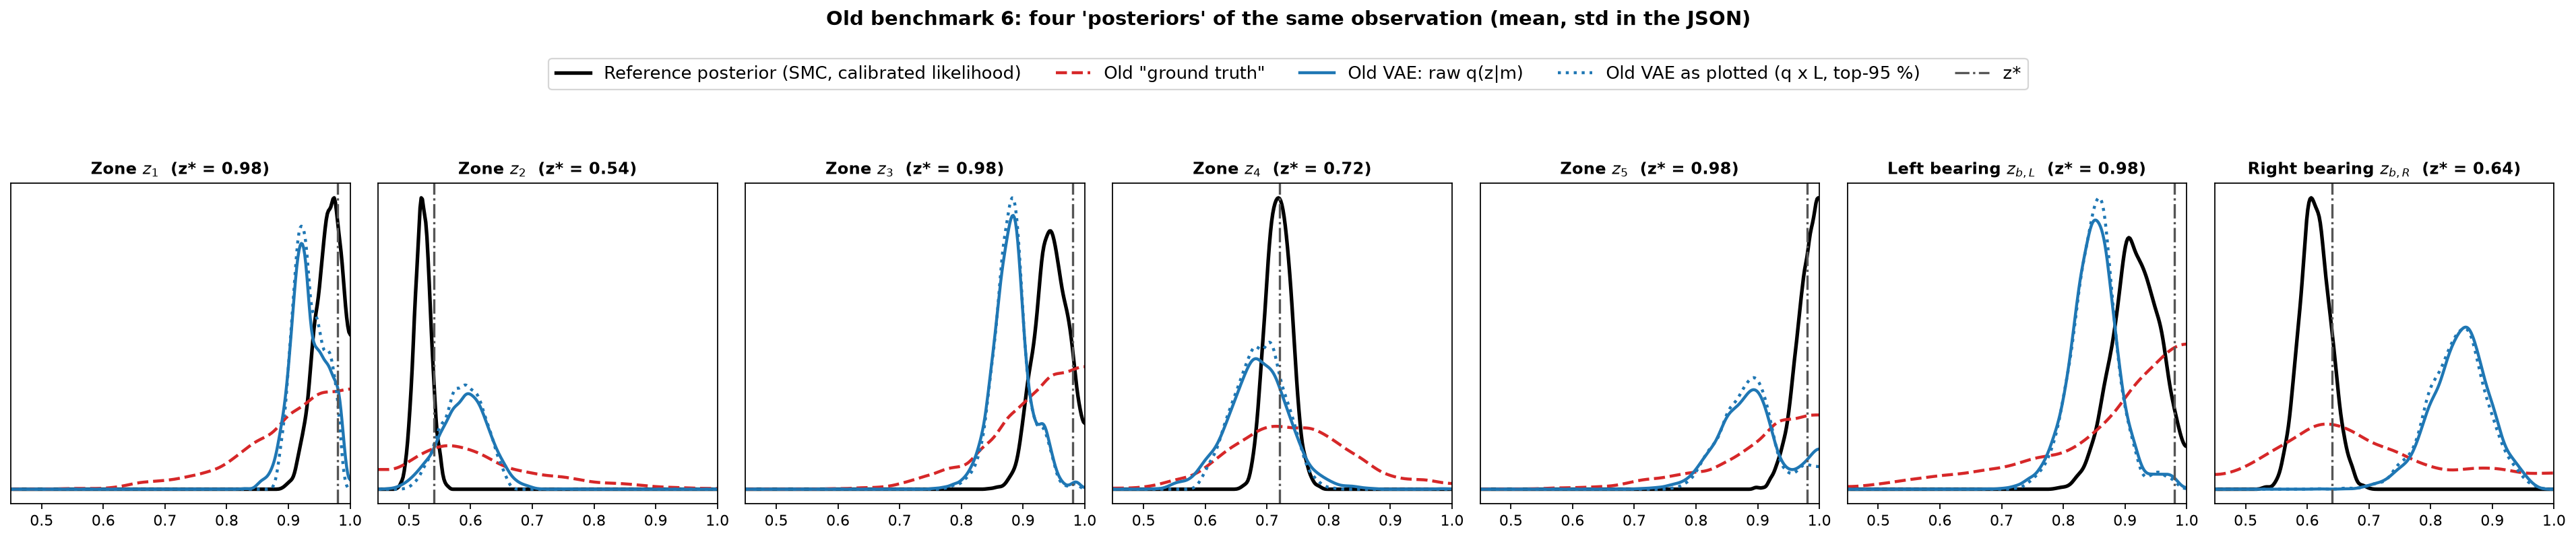
\includegraphics[width=\textwidth]{figures/Fig_old_vs_reference_P6.png}\caption{}\end{subfigure}
\caption{Diagnosis of the previous implementation. (a) The PDF term remains at its clipping limit, the copula
correlation matrices are nearly singular, and the posterior means are biased. (b) Four estimates of the posterior of
the same observation (benchmark 6): exact posterior (black), previous reference (red, dashed), previous VAE (blue) and
previous VAE as plotted after re-weighting (blue, dotted).}
\label{fig:old}
\end{figure}

\subsection{Corrected loss function}

The loss keeps the structure of Eq.~(10). The difference lies in the weights of the frequency and MAC terms: instead of
fixed values, they are now given by the calibrated statistics of the discrepancy between observations and decoder
(Eq.~\ref{eq:discrepancy}):
\begin{equation}
\begin{split}
\Lelbo(\bm\theta) = {} & \underbrace{\frac{1}{N H}\sum_{i=1}^{N}\sum_{h=1}^{H}
\tfrac12\,\mathbf{d}_{ih}^{\top}\bm\Sigma_f^{-1}\mathbf{d}_{ih}}_{\mathcal{L}_{\mathrm{freq}}}
+\underbrace{\frac{1}{N H}\sum_{i=1}^{N}\sum_{h=1}^{H}\sum_{j=1}^{n_m}
\frac{1-\mathrm{MAC}_j(\bm\Phi_i,\hat{\bm\Phi}_i^h)}{2s_{v,j}^2}}_{\lambda\mathcal{L}_{\mathrm{MAC}}} \\
& +\gamma^2\,\underbrace{\frac1N\sum_{i=1}^N \mathbb{E}_q\big[\log q_{\bm\zeta_{\bm\theta}}(\z|\m_i)\big]}_{\mathcal{L}_{\mathrm{PDF}}},
\end{split}
\label{eq:elbo}
\end{equation}
where $\mathbf{d}_{ih}=\log\f_i-\mathbf{b}-\log\hat{\f}_i^h$. For unit-norm mode shapes perturbed by Gaussian noise,
$1-\mathrm{MAC}$ equals the squared noise component perpendicular to the shape, so the MAC term is the Gaussian
log-likelihood of that noise and does not depend on the sign of the modes. With these weights and a uniform prior,
Eq.~\eqref{eq:elbo} is the negative ELBO and its minimizer is the Bayesian posterior when $\gamma=1$; other values of
$\gamma$ produce tempered posteriors and are selected on the validation set. We compute the PDF term through the
entropy of the copula model,
\begin{equation}
\mathbb{E}_q[\log q] = -\tfrac12\log\det\bm\Sigma - \sum_{e=1}^{7} H[q_e],
\label{eq:entropy}
\end{equation}
where the copula part is exact and the entropies of the marginals $q_e$ are estimated with the $H$ samples. This
reduces the variance of the estimate compared with evaluating $\log q$ at the samples. The penalty that pushed samples
away from the bounds and the term that forced diverse mixture weights were removed, since both shifted the optimum
away from the posterior.

\subsection{Sampling layer and training}

The Kumaraswamy-mixture marginals are sampled by inverting their cumulative distribution function at the uniform
variables produced by the Gaussian copula. The gradients of the samples with respect to the encoder outputs are
computed exactly through the implicit function theorem, without clipping; they agree with finite differences to a
relative error of $7\times10^{-6}$. Table~\ref{tab:training} lists the training specifications. During the first 150
epochs, the data terms are multiplied by a factor that grows from 0.01 to 1, so that the approximate posterior first
covers the plausible region and then concentrates on it. The model with the lowest validation loss after this warm-up
is retained.

\begin{table}[H]
\centering\small
\caption{Training specifications.}
\label{tab:training}
\begin{tabular}{p{4.2cm}p{10.6cm}}
\toprule
Encoder & three hidden layers (128, 256 and 128 neurons), ReLU, He uniform initialization \\
Approximate posterior & Gaussian copula with Kumaraswamy-mixture marginals ($K=3$) on $[0.45,1]$ \\
Samples per observation & $H=6$ \\
Optimizer & Adam, cosine learning rate from $5\times10^{-4}$ to $10^{-5}$, batch size 256 \\
Warm-up & data terms multiplied by a factor growing from 0.01 to 1 over the first 150 epochs \\
Epochs and model selection & 1\,500 epochs; lowest validation loss after the warm-up \\
Hyperparameter $\gamma$ & $\gamma=1$ (Bayesian posterior) \\
Hardware & 16-thread CPU, 3--4 s per epoch \\
\bottomrule
\end{tabular}
\end{table}

\subsection{Verification of the corrected code}

We first verified the corrected code on the intermediate dataset (five-element model, frequencies and both vertical and
rotational mode shapes), whose exact posteriors are narrow and therefore demanding in terms of accuracy. After 1\,500
epochs, the VAE reproduces the exact posteriors of the eleven benchmark scenarios (Fig.~\ref{fig:verif}). The median
ratio between the standard deviations of the VAE and of the exact posterior is 1.02, the mean difference between their
means is 0.002, and the true damage condition is contained in the 95\% credible intervals of 94\% (zones) and 93\%
(bearings) of the test parameters, compared with 72\% for the previous implementation. Figure~\ref{fig:loss} shows the
evolution of the loss and of each of its terms.

\begin{figure}[H]
\centering
\begin{subfigure}{0.49\textwidth}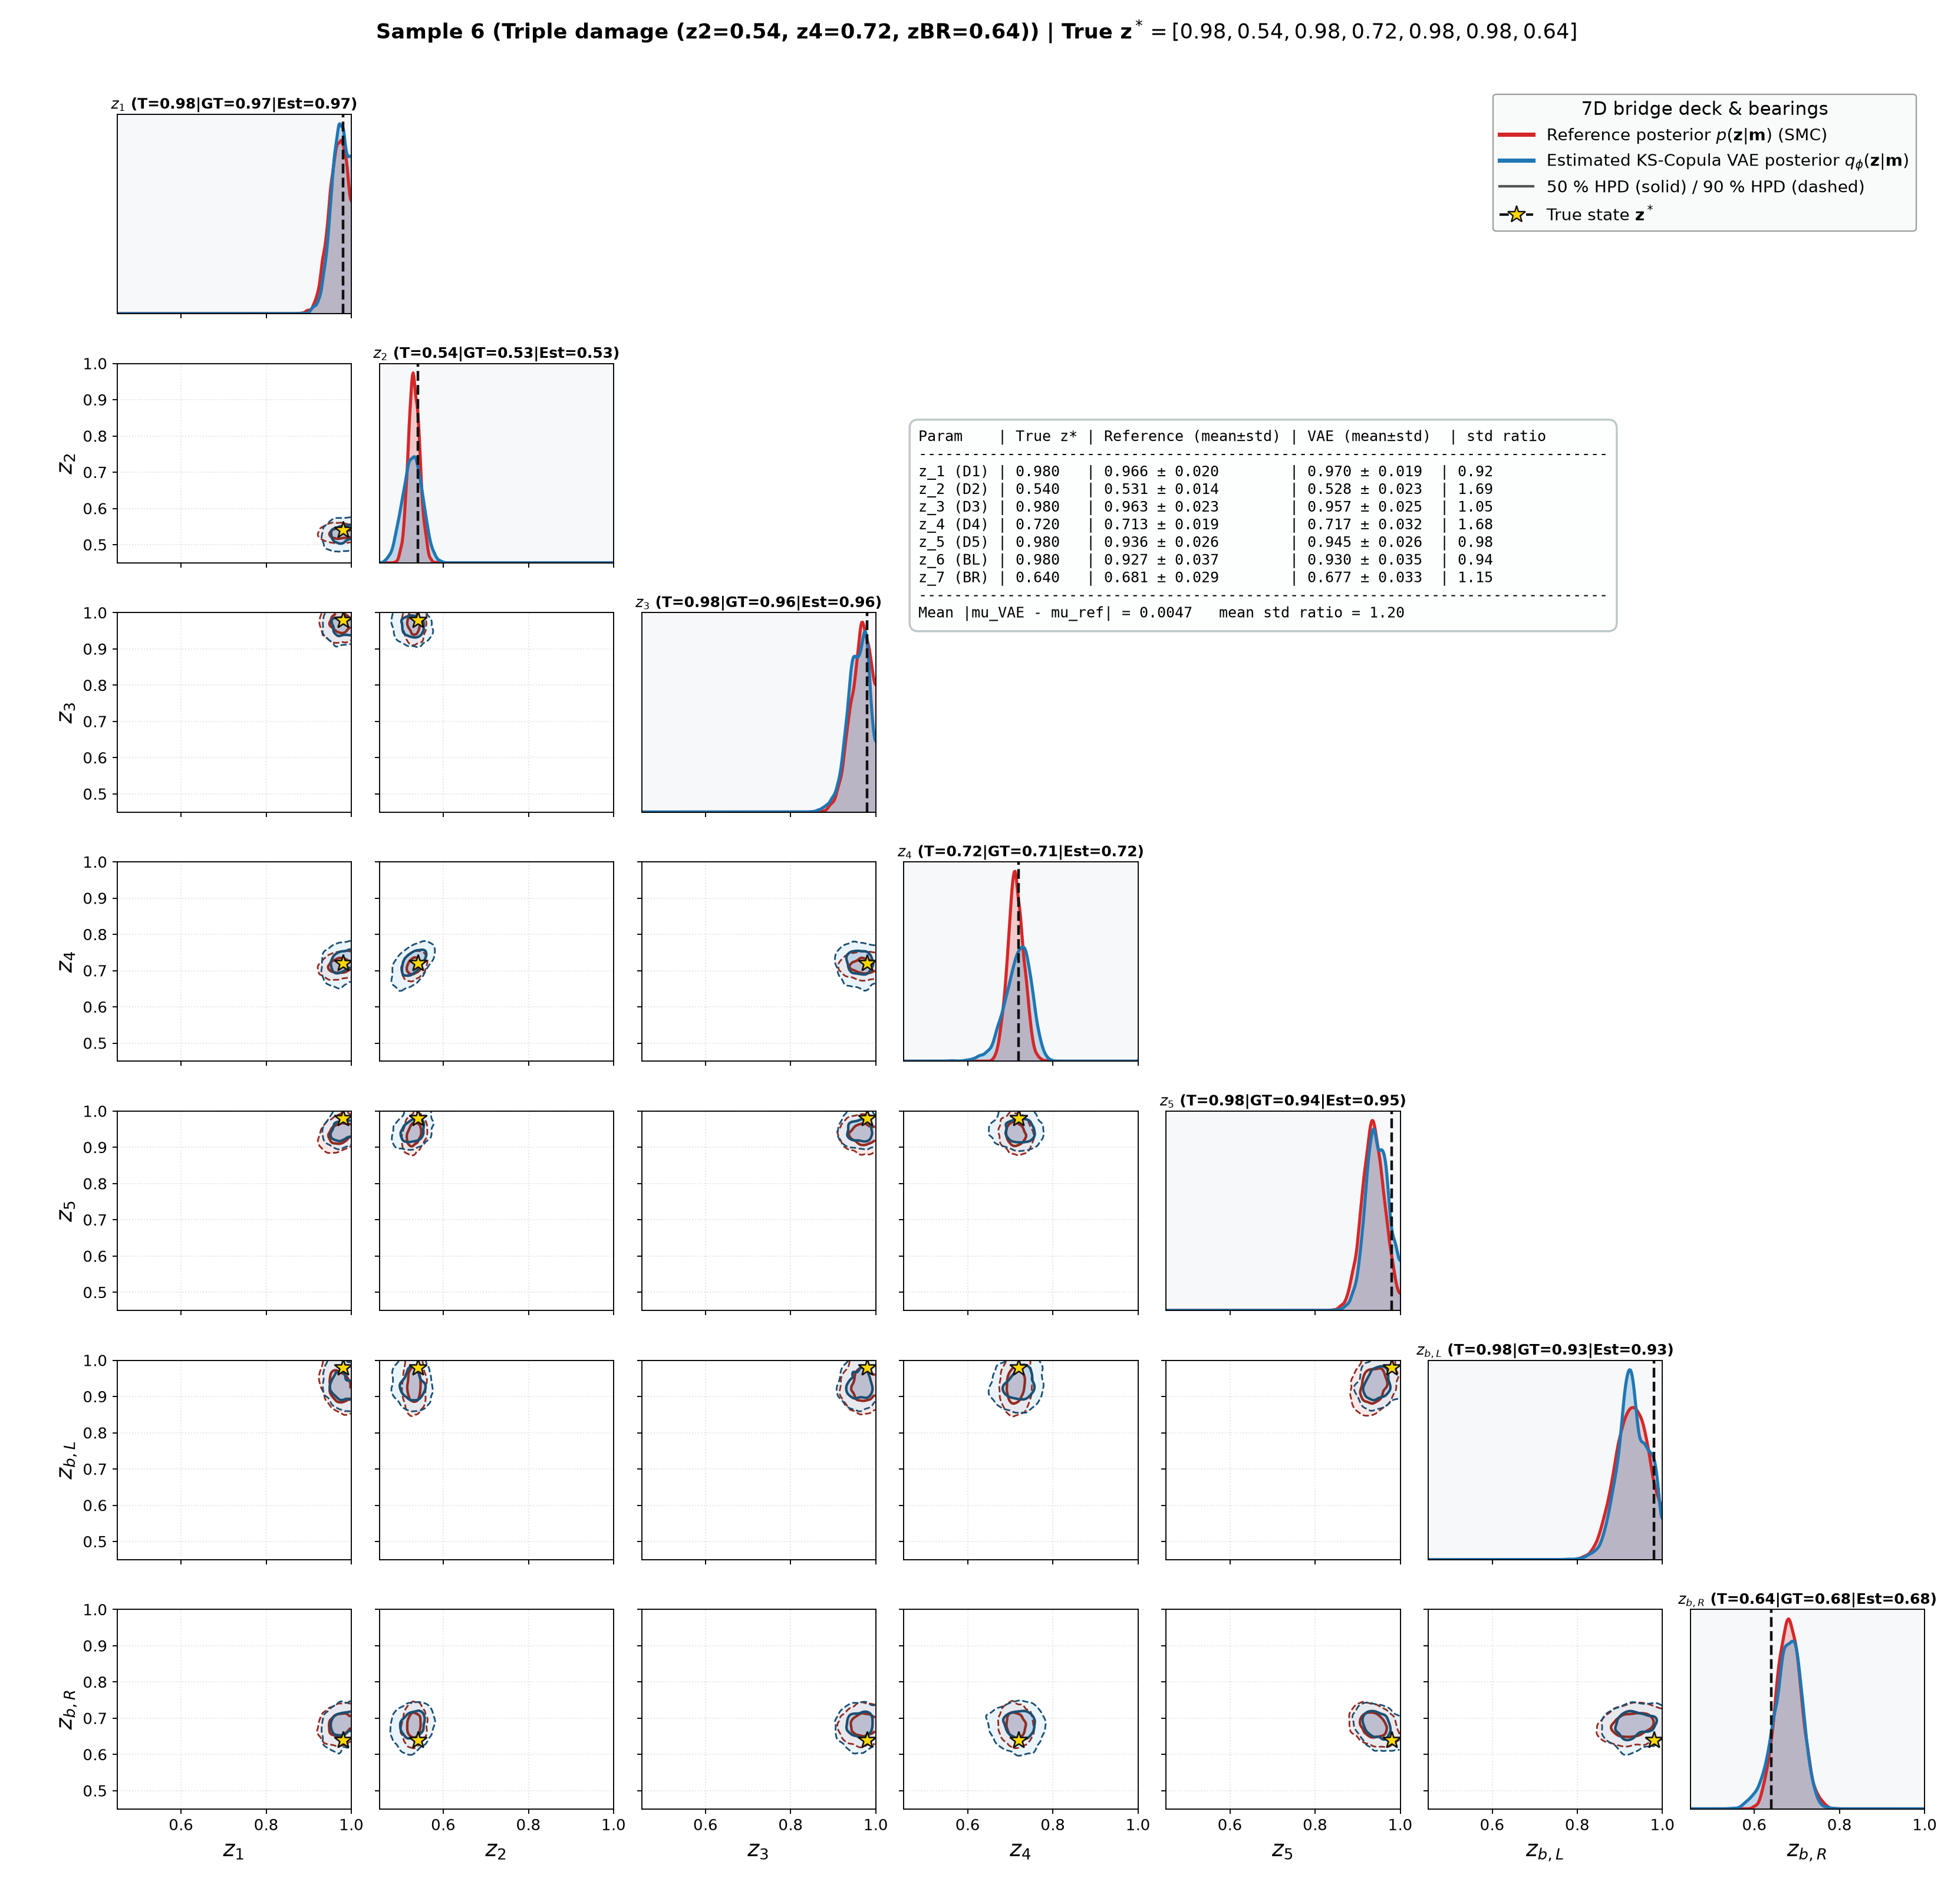
\includegraphics[width=\textwidth]{figures/Verif_P6_Overlay.png}\caption{Benchmark 6}\end{subfigure}
\begin{subfigure}{0.49\textwidth}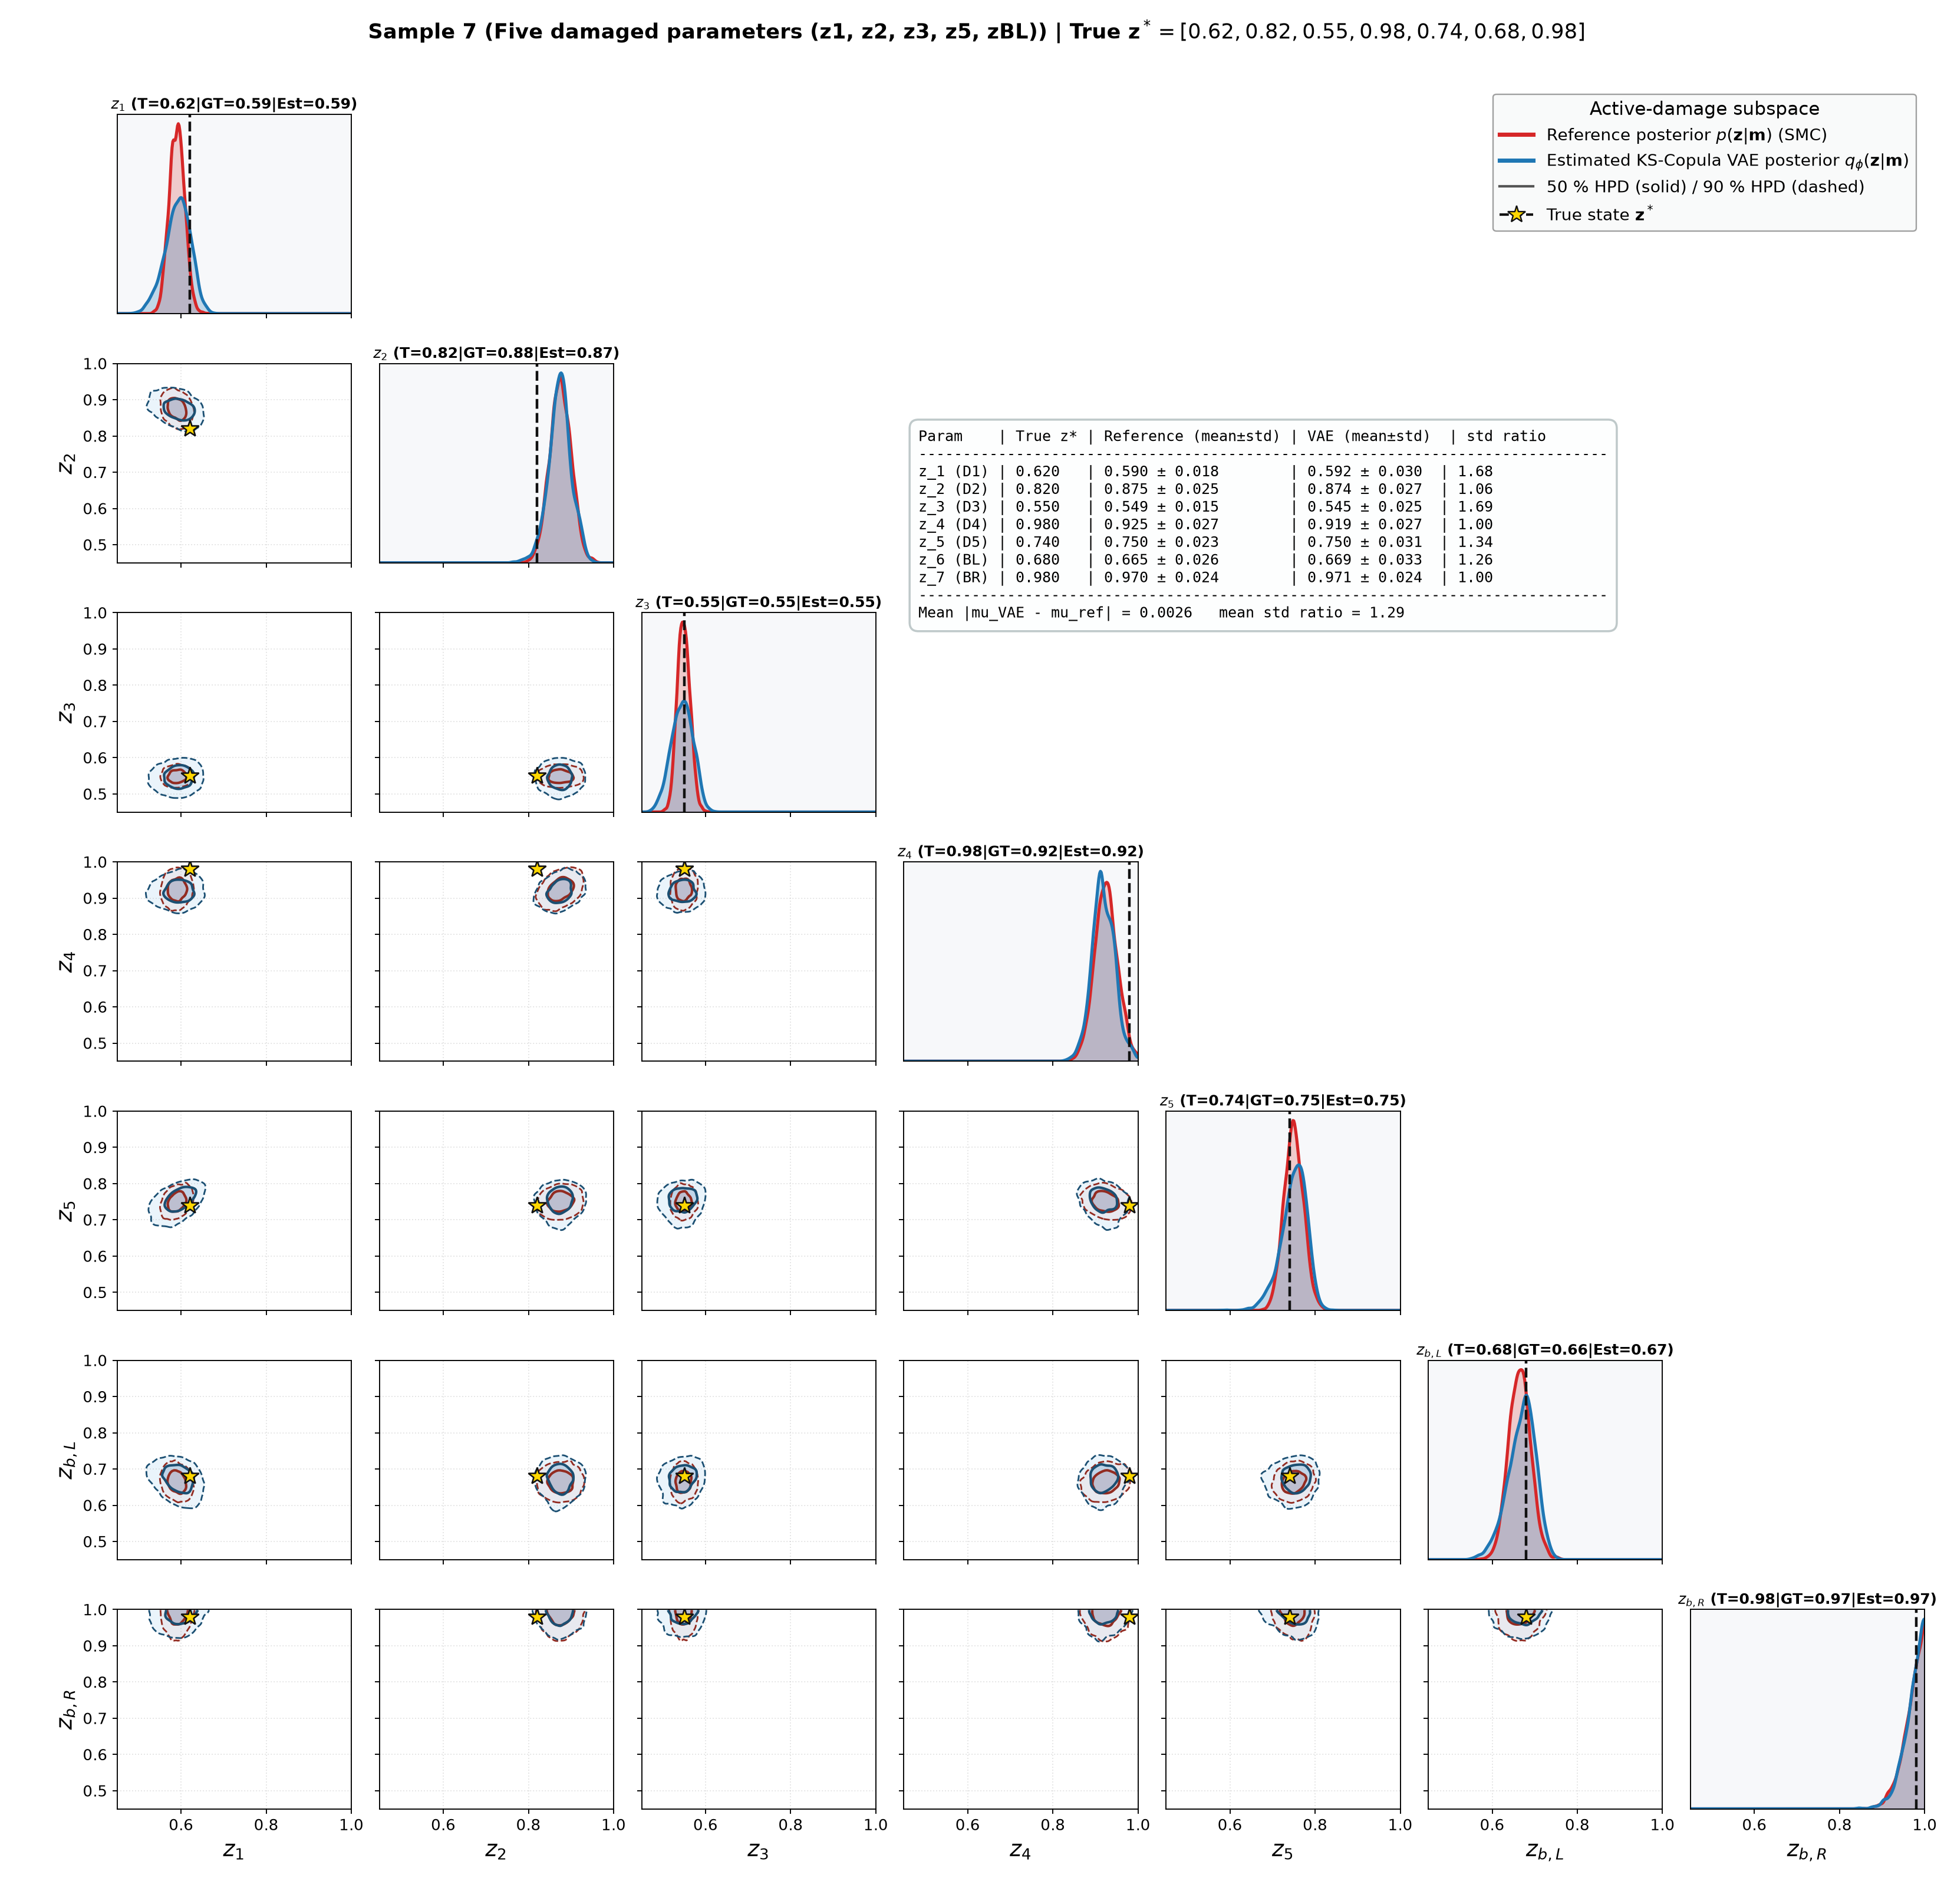
\includegraphics[width=\textwidth]{figures/Verif_P7_Active.png}\caption{Benchmark 7 (damaged parameters)}\end{subfigure}\\[4pt]
\begin{subfigure}{0.53\textwidth}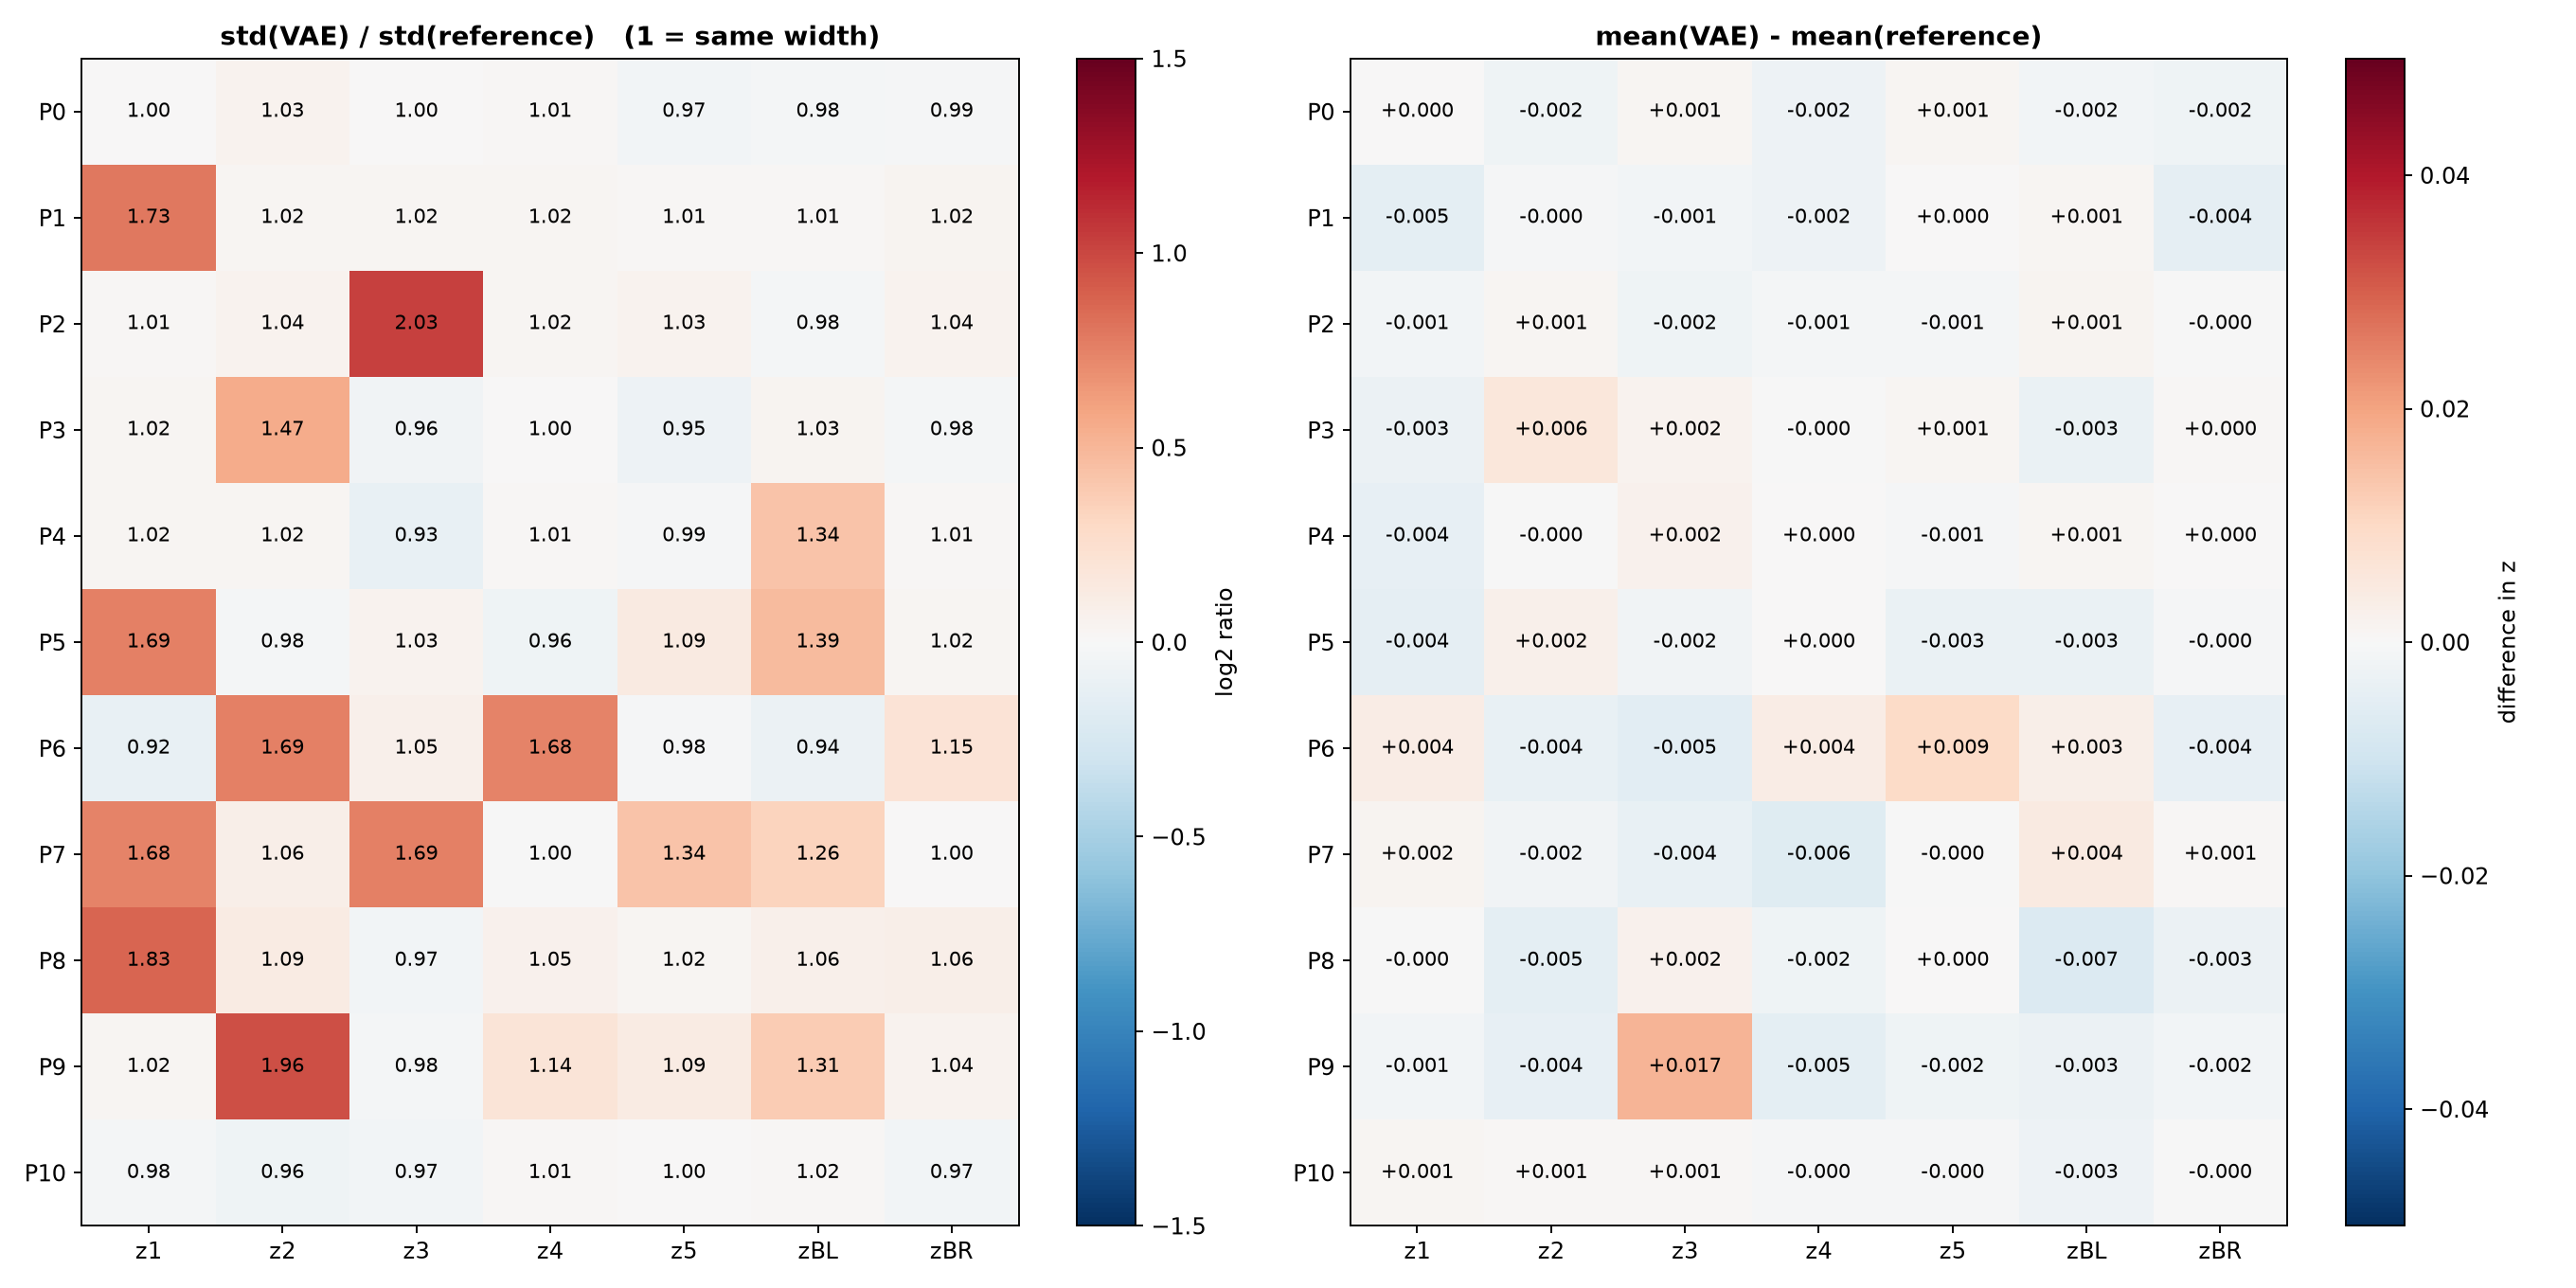
\includegraphics[width=\textwidth]{figures/Verif_benchmark_summary.png}\caption{Ratio of standard deviations and difference of means}\end{subfigure}
\begin{subfigure}{0.44\textwidth}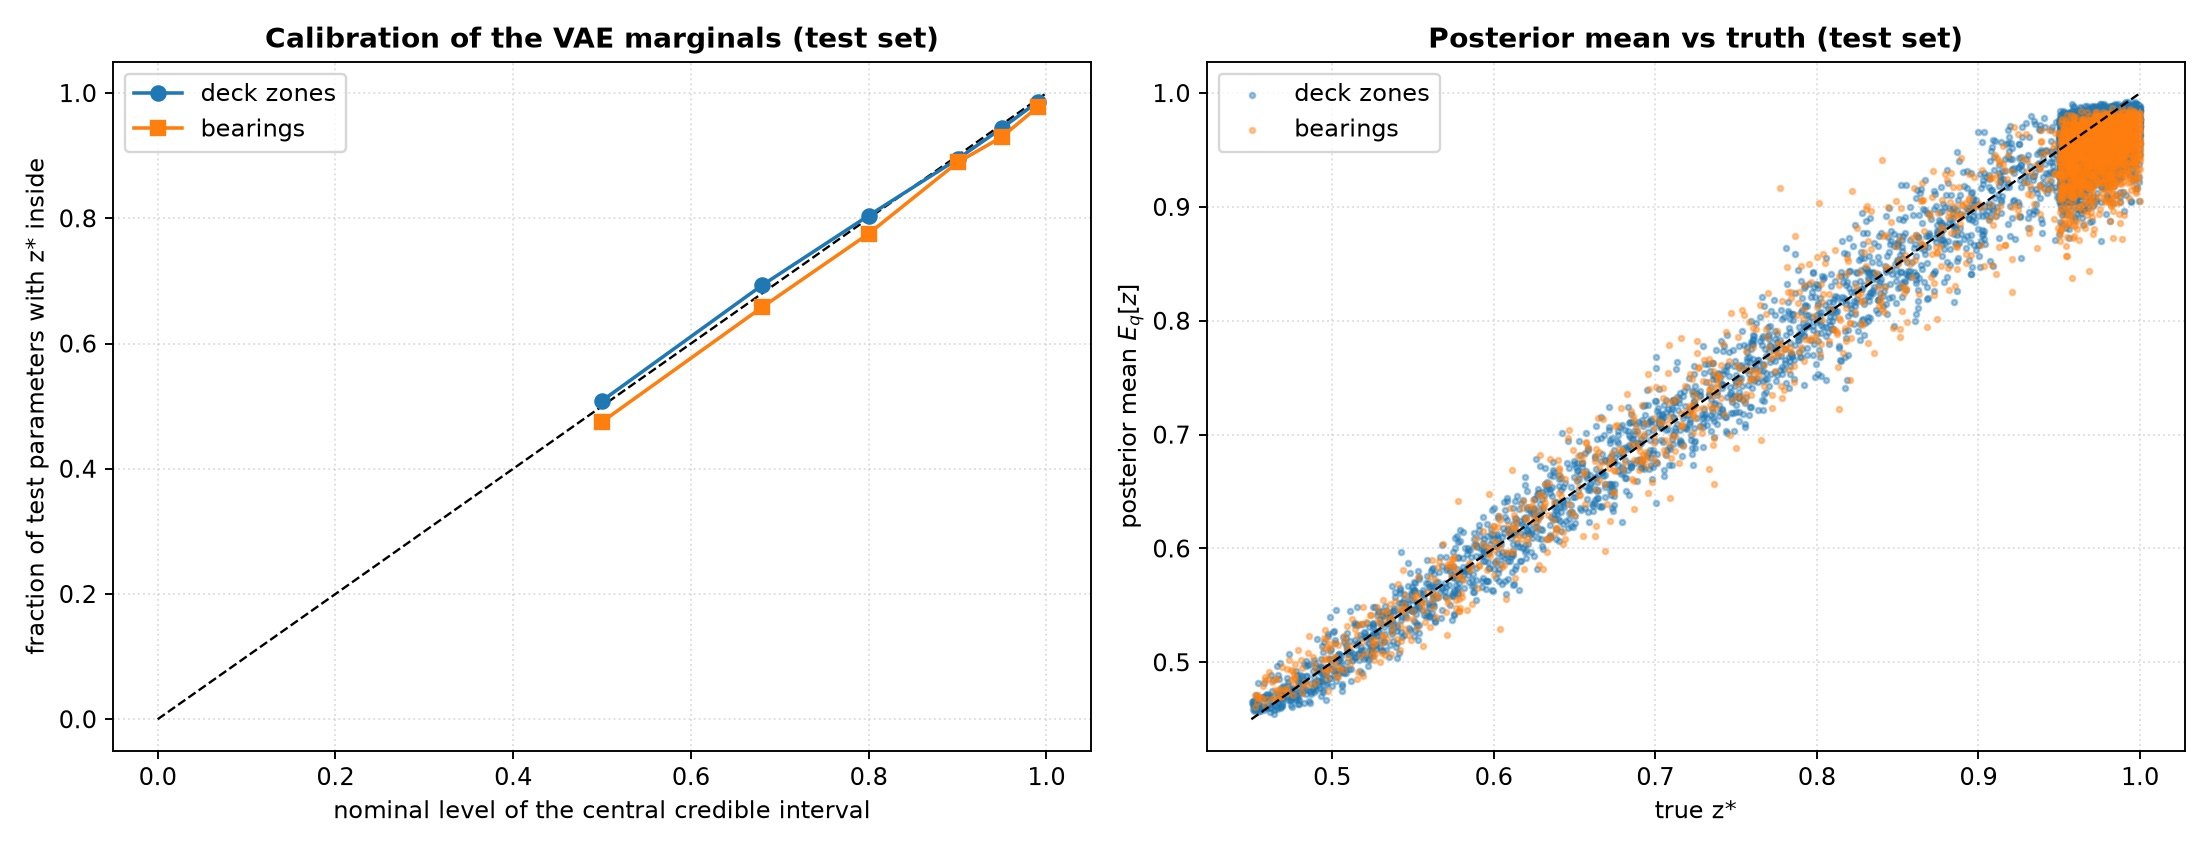
\includegraphics[width=\textwidth]{figures/Verif_calibration.png}\caption{Coverage and posterior means over the test set}\end{subfigure}
\caption{Verification of the corrected code on the intermediate dataset: exact posterior (red) and VAE posterior
(blue); solid and dashed contours enclose 50\% and 90\% of the probability.}
\label{fig:verif}
\end{figure}

\begin{figure}[H]
\centering
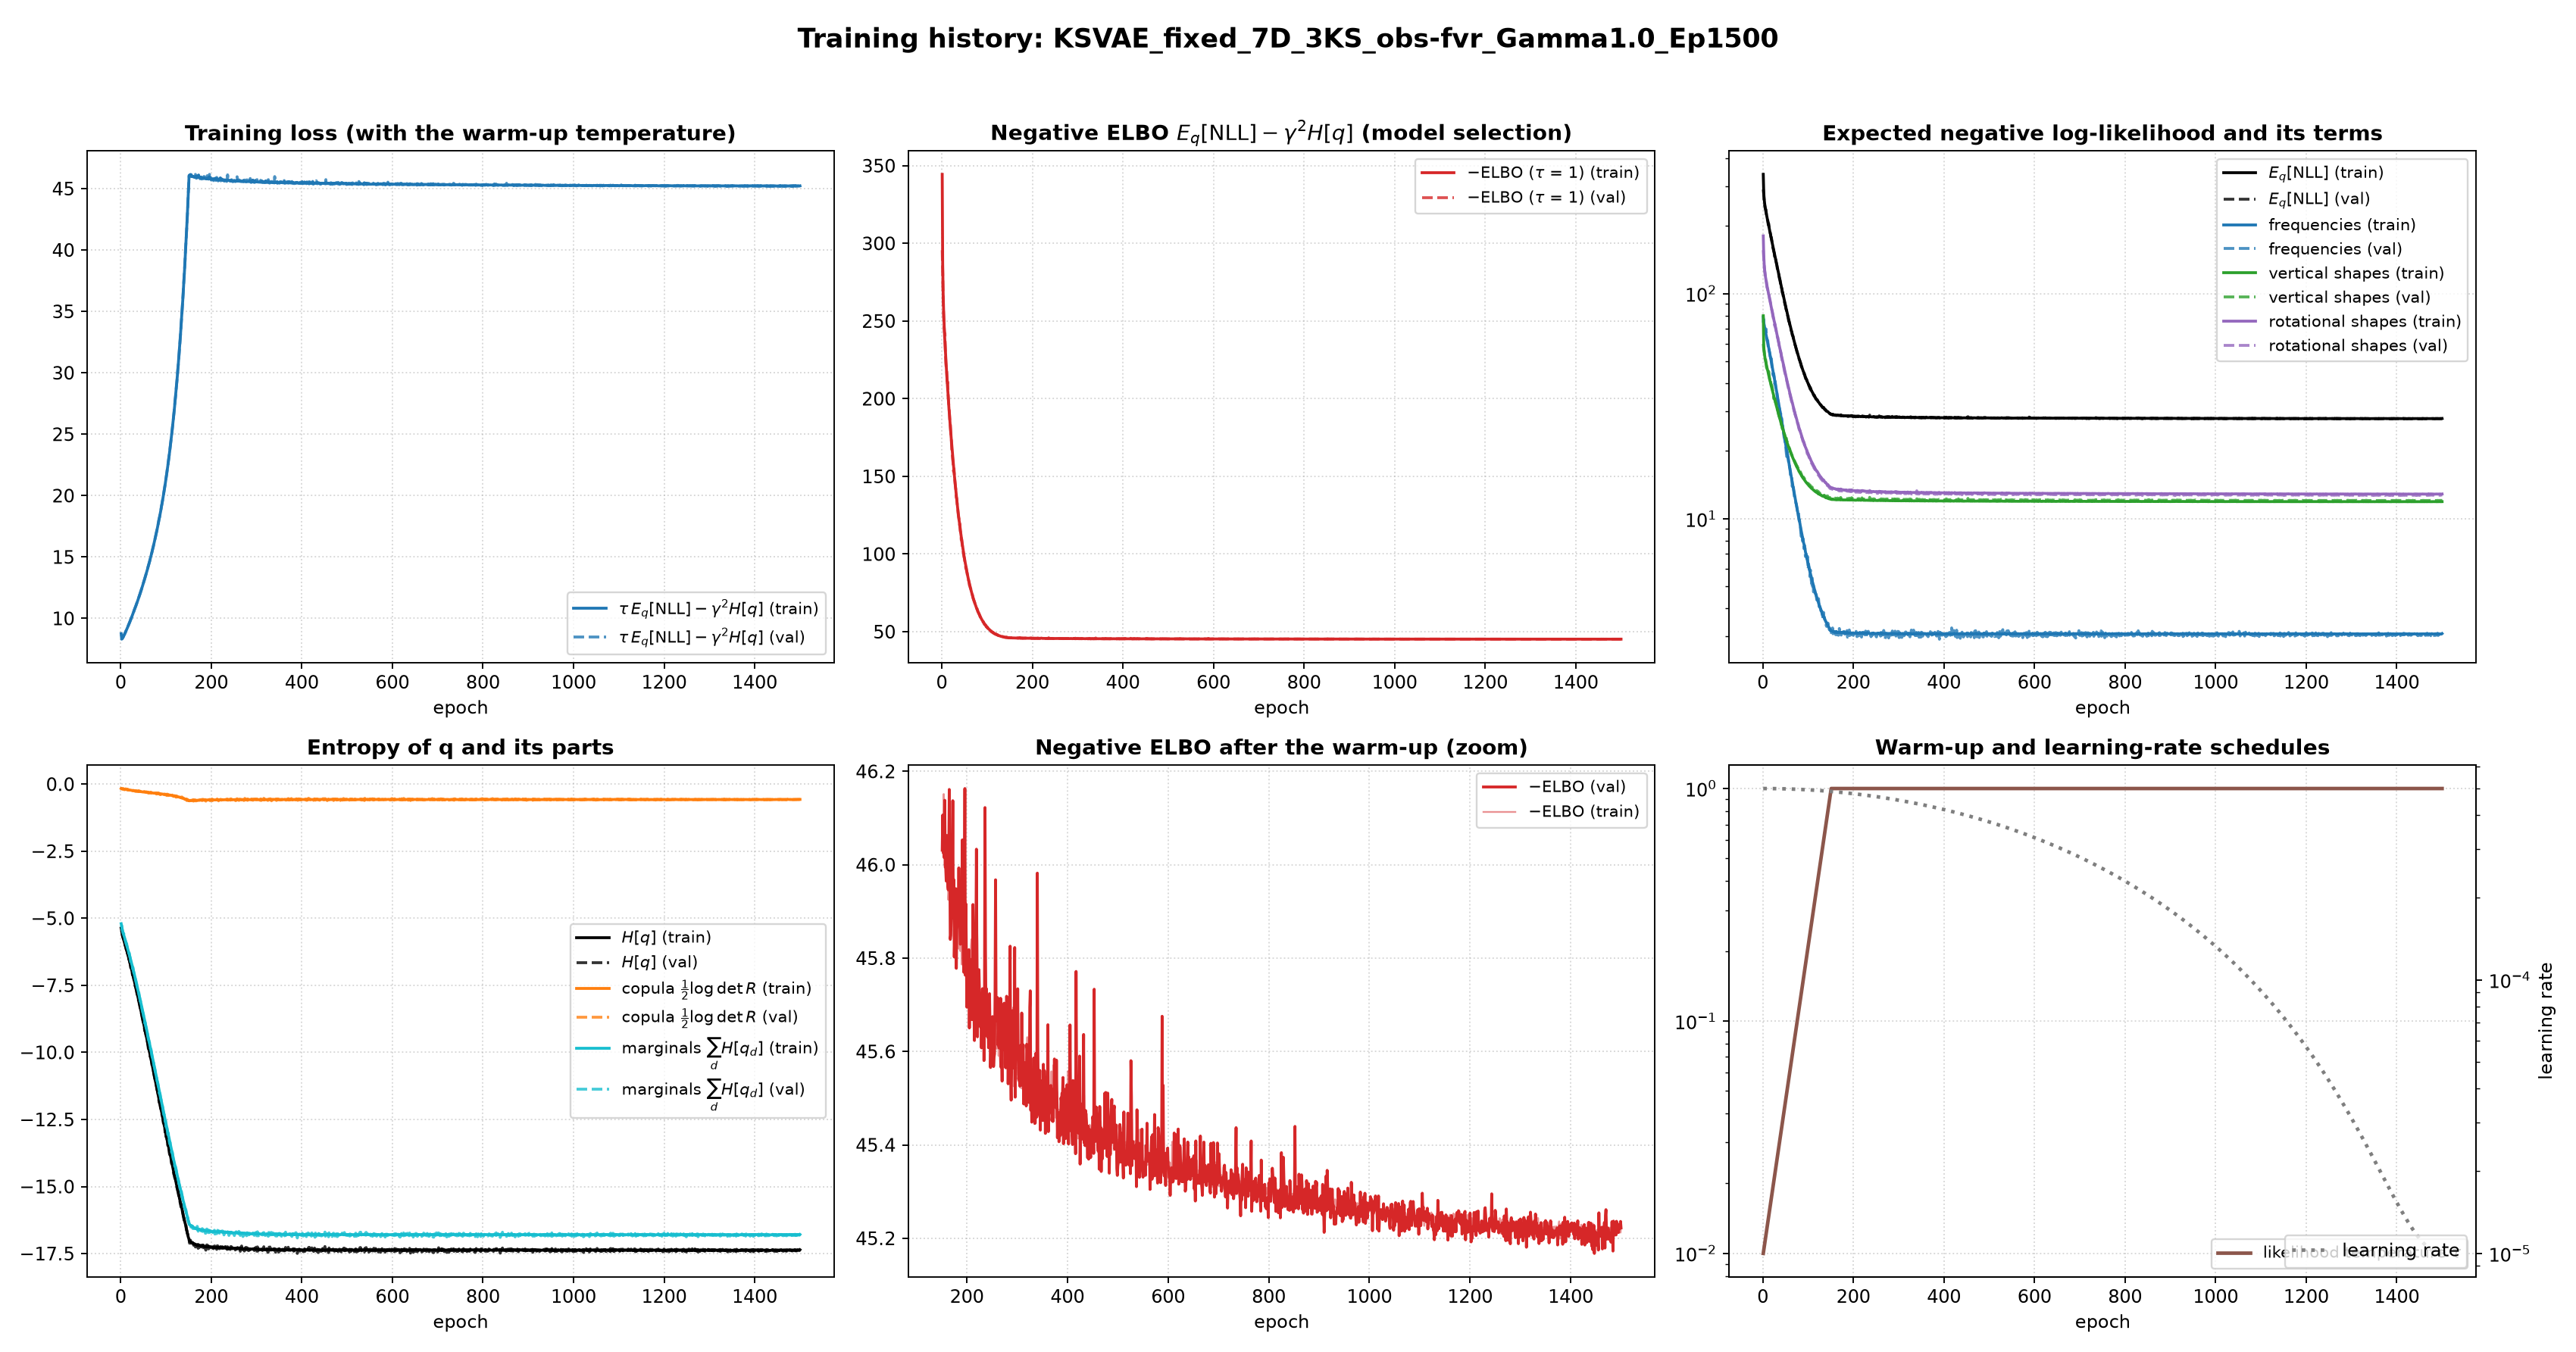
\includegraphics[width=\textwidth]{figures/Verif_Training_Loss_Curves.png}
\caption{Evolution of the loss and its terms for training and validation data.}
\label{fig:loss}
\end{figure}

\textcolor{red!70!black}{The results of the VAE trained on the final dataset (Fig.~\ref{fig:gt}) will be added when
the corresponding training finishes.}

% =============================================================================
\section{Post-processing and reference posterior}
% =============================================================================

\subsection{Exact posterior of the test scenarios}

To assess the VAE, we need the exact posterior of each benchmark observation $\m_t$ under the same model that the VAE
targets: the same decoder, the same calibrated likelihood and the same prior,
\begin{equation}
p(\z|\m_t)\propto\exp\!\big(-\mathrm{NLL}(\z;\m_t)\big)\,\mathcal{U}(\z;\mathcal{S}),
\end{equation}
where $\mathrm{NLL}$ is the data part of Eq.~\eqref{eq:elbo} for a single sample. We draw 4\,000 samples from this
distribution with sequential Monte Carlo (SMC), which does not use the true damage condition at any stage. The
algorithm starts from samples of the prior and introduces the likelihood gradually through an exponent $\beta$ that
grows from 0 to 1. At each step, $\beta$ is increased as much as possible while keeping half of the samples effective,
the samples are resampled according to their weights, and each of them is moved with random-walk Metropolis steps that
leave the current tempered distribution invariant. Each benchmark requires 7--10 steps and 10--20 seconds on a
CPU. Two independent runs give the same posterior (Wasserstein distance below 0.0013 per parameter), and a
brute-force importance sampling with two million prior samples reproduces the SMC means and standard deviations within
0.002.

\subsection{Comparison between estimated and exact posteriors}

The VAE posterior of a test observation is represented by 4\,000 samples drawn from $q_{\bm\zeta_{\bm\theta}}(\z|\m_t)$,
without any further processing. Both posteriors are displayed with the same kernel density estimator, which accounts
for the bounds of $\mathcal{S}$, and the joint densities are shown through the contours that enclose 50\% and 90\% of
the probability. For each benchmark, we compare the means, the standard deviations and the correlations of both
posteriors and compute the Wasserstein distance between their marginals. Over the whole test set, we compute the
central credible intervals of the exact VAE marginals at nominal levels between 50\% and 99\%, their coverage of the
true damage condition, their width, the error of the posterior mean, and the false-alarm rate on undamaged parameters.

\subsection{Procedure}

All steps are run from the project root (see \texttt{README.md}):
\begin{enumerate}[leftmargin=*]
\item \texttt{dataset\_generation.py} generates the datasets, calibrates the likelihood and plots the data figures.
\item \texttt{check\_consistency.py} runs numerical checks of the likelihood, the sampling layer and the calibration.
\item \texttt{reference\_posterior.py} computes and stores the exact posteriors of the benchmark scenarios.
\item \texttt{main\_train\_KSVAE.py} trains the VAE and stores the posterior parameters of the test set.
\item \texttt{postprocessing.py} produces the loss curves, the coverage analysis, the corner plots and the metrics.
\end{enumerate}

\end{document}
